\chapter{Design Approach and Solutions}
\label{design-approach}
Due to the complexity of the system and highly interconnected setup of components, the design process throughout both quarters was a fast-paced, highly iterative design process that saw hundreds of models produced and dozens tested. The following sections detail the initial design and development of each component on the alpha prototype.

\section{Initial Research, Testing and Prototype Development}
Prior to dividing the prototype into 3 distinct, but communicating systems, research was conducted for various options for propulsion and deployment mechanisms. 

\subsection{Propulsion Selection}
Most traditional rocket landing systems use a gimballed thrust vector control system together with a combustion based engine to land the rocket (see Section \ref{competitive-analysis}). However, one of our client's requirements was that combustion not be used to land the rocket. This also ties in with the needs and specifications outlined in Section \ref{needs-and-specs}, specifically need \#10 which states that the product must follow competition guidelines, and one of the guidelines specifically prohibits the use of explosive materials during landing. With this requirement in mind, the team set out researching a variety of different propulsion methods ranging from water jets to ducted fans. 

One of the solutions that was analyzed was the concept of cold gas thrust. Cold gas thrust is already commonplace in the aerospace industry and it would potentially allow us to use existing infrastructure. Despite its potential, cold gas is almost exclusively used for minor trajectory corrections or slowly propelling astronauts on space walks, never for outright propulsion. To determine whether or not cold gas thrust could work for our client's purposes, an computational fluid dynamics simulation using ANSYS Fluent was conducted to determine the feasibility of this solution. It was found that using this form of propulsion would require the addition of up to 15kg of compressed gas, tanks, and regulators the system, rendering it completely unfeasible. For more information on this simulation, please see Appendix \ref{app:cold-gas-thruster}.

After this calculation was completed, the team was able to narrow in on the propulsion front runners through the use of an alternatives matrix (figure \ref{fig:PAM}). After more in depth research on minimum sizes and maximum thrusts of the front runners, the team proceeded with a quadcopter style propulsion system in which four motors would be mounted in a square pattern and would be controlled by an onboard avionics suite. 

\begin{figure}[H]
    \centering
    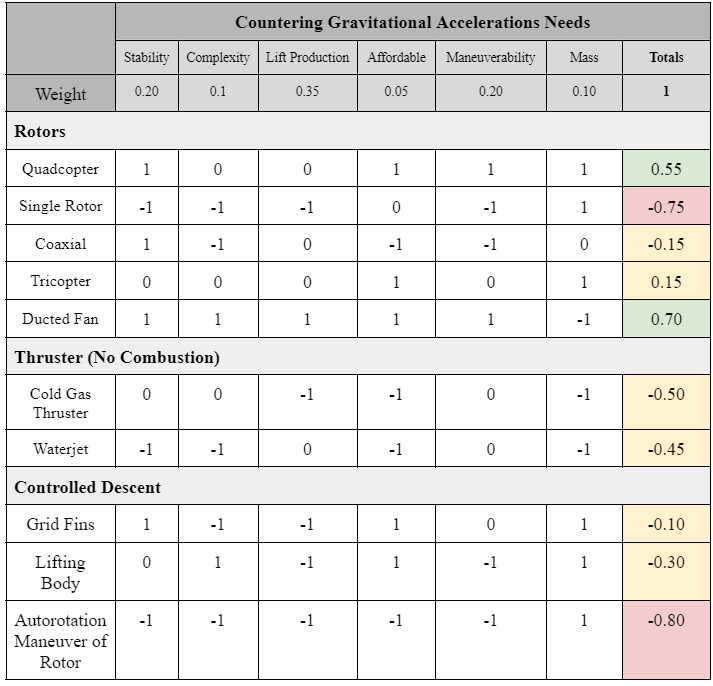
\includegraphics[width=0.5\textwidth]{src/figs/AltProp.png}
    \caption{Propulsion Alternative Matrix}
    \label{fig:PAM}
\end{figure}

\subsection{Deployment Research and Development}
Deciding to go with a propeller based system provided the team with a new challenge to navigate; these four propellers now had to be able to be stowed inside a cylinder that is a smaller diameter than they are. In order to accomplish this, the arms would need to be fixed at some point in the body and swing out to their deployed position. Design focus quickly shifted to developing this system so it could be tested and iterated. The initial idea was the use of 4 servos, one on each arm that would actuate the arm 90 degrees to its deployed position. This method was tested using a light servo that was believed to have enough torque to deploy the arm. However, it was quickly found that the servo purchased could not move the arm as fast as we needed it to and increasing the torque of the servo was not an option because of size and mass constraints. 

The team began looking into deployment methods that could use one centralized servo to deploy all four arms simultaneously. Initial ideas involved the use of a complex gear system to take rotation from the servo and change its rotation direction to deploy the arm 90 degrees. This idea was quickly written off due to its mechanical complexity. The other leading deployment option was through the use of torsion springs. Torsion springs provided a lightweight, reliable and fast solution to deploy the arms from inside the rocket body. 

In order for torsion springs to work, a mechanism to keep the arms inside the rocket also had to be developed. With the teams goal of finding a solution that allowed the use of one actuator to control four components, the idea of a centrally located unlocking disk emerged. This disk would have 4 protrusions that blocked the arms from deploying from the rocket. When thrust was needed, the disk would rotate via a single servo. This would move the protrusions from the arms path of travel, allowing the torsion springs to push them to their deployed position.

Once the unlocking system had been designed, an accompanying arm was designed that had a small rectangular protrusion on the motor end that would interface with the unlocking disk while the arm was stowed. 

These components were all printed or purchased and combined to form the teams critical system prototype the Arm Deployment Test Stand (ADTS). The image of the original ADTS is shown in figure \ref{fig:ADTS}. The following sections detail the design process since the quarter 1 critical system prototype delving into changes made to the ADTS system as well as the component creation and iteration.

\section{Motors and Blade Selection}
\label{design:motors-selection}
Once the team had decided on using propellers for the propulsion mechanism, the next step was to select the appropriate motor and blade to generate the thrust required to slow down and maneuver the rocket while it's falling. For this the team made heavy use of the Static Thrust Stand (STS) that was constructed during Quarter 1. Although a simulation driven approach to motor and propeller selection could have been attempted using various computational fluid dynamics packages such as ANSYS Fluent, it was determined that a quicker and more accurate approach would be to obtain empirical data for thrust generated by different motor and blade combinations using the STS. The static thrust stand, pictured in Figure \ref{design:STS}, features a load cell, load cell amplifier, Raspberry Pi computer, and electronic speed controller (ESC) which work together to log thrust values produced by the motor/propeller that is mounted to the load cell. The data is then saved and plotted which serves as an excellent way to determine what the ideal motor and blade combination will be. Furthermore, the Python code used for the STS can be found in Appendix \ref{app:sts-code}.

\begin{figure}[H]
    \centering
    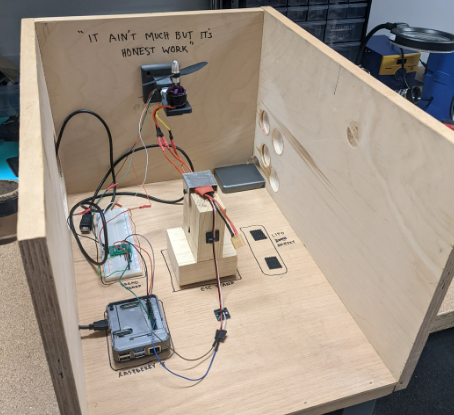
\includegraphics[width=0.75\textwidth]{src/figs/STS.png}
    \caption{Static Thrust Stand (STS)}
    \label{design:STS}
\end{figure}
Figure \ref{design:diff_blades} shows the thrust produced by several different blade sizes with the same motor. The team determined early on that the primary factor that affects thrust is the blade diameter, while pitch and blade shape have a less significant effect.
\begin{figure}[H]
    \centering
    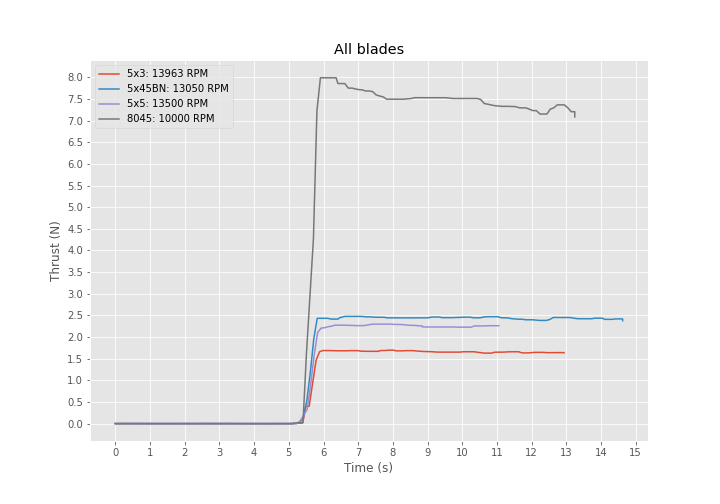
\includegraphics[width=0.85\textwidth]{src/figs/STS_4_diff_blades.png}
    \caption{Comparison of thrust for different blades}
    \label{design:diff_blades}
\end{figure}

Initial mass estimates of the final fully assembled rocket dictated the amount of the thrust that would be needed to stop and land the rocket. Further calculations to determine an acceptable thrust to weight ratio were conducted as well and can be found in Section \ref{thrust_analysis}. At this stage, the team began by testing several different motors and blades. First, in an effort to achieve the highest possible RPM, several high kv (RPM/volt), low stator size motors were tested to see if they would give ample thrust. Plots from the static thrust can be seen in Figures \ref{design:sts:2450} and \ref{design:sts:2550}. Unfortunately, these motors were not a good choice since the low stator size equates to lower torque capabilities. This is evident from the plots of thrust versus time since the thrust continually decayed as time went on. Additionally, over-torquing the motors resulting in lots of excess heat being generated outside of nominal operating temperatures.
\begin{figure}[H]
    \centering
    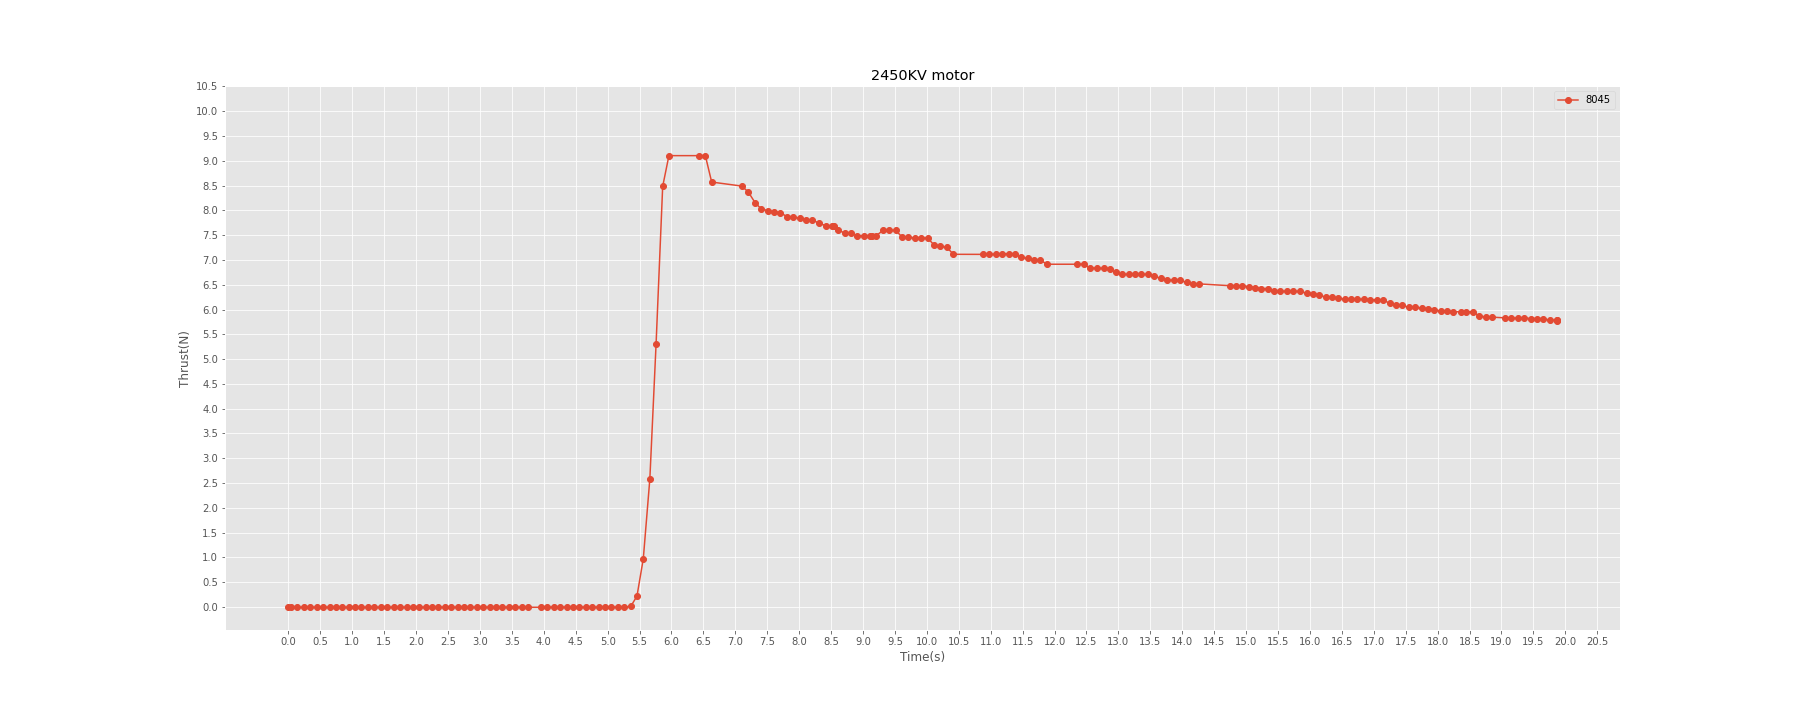
\includegraphics[width=\textwidth]{src/figs/small_2450_motor.png}
    \caption{2450 KV motor}
    \label{design:sts:2450}
\end{figure}

\begin{figure}[H]
    \centering
    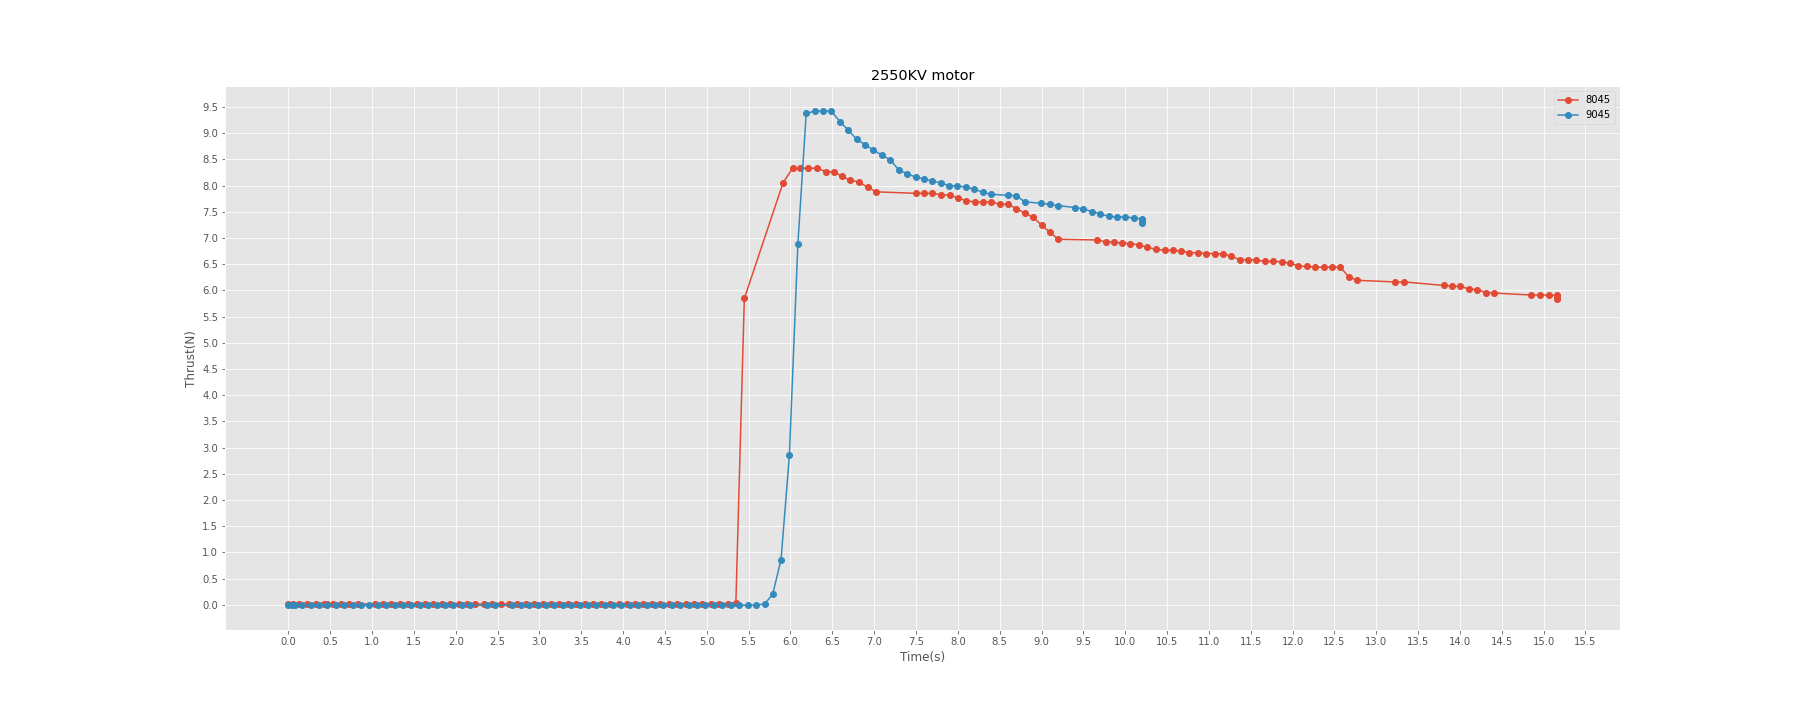
\includegraphics[width=\textwidth]{src/figs/small_2550_motor.png}
    \caption{2550 KV motor}
    \label{design:sts:2550}
\end{figure}
Once it was determined that higher torque motors were needed, the team tested some larger stator size motors with several different blades and were very pleased with the results. The larger motors were capable of outputting the torque needed to spin the blades at speed while also producing substantial thrust. The thrust versus time plot for this new motor is shown in Figure \ref{design:sts:purple}.
\begin{figure}[H]
    \centering
    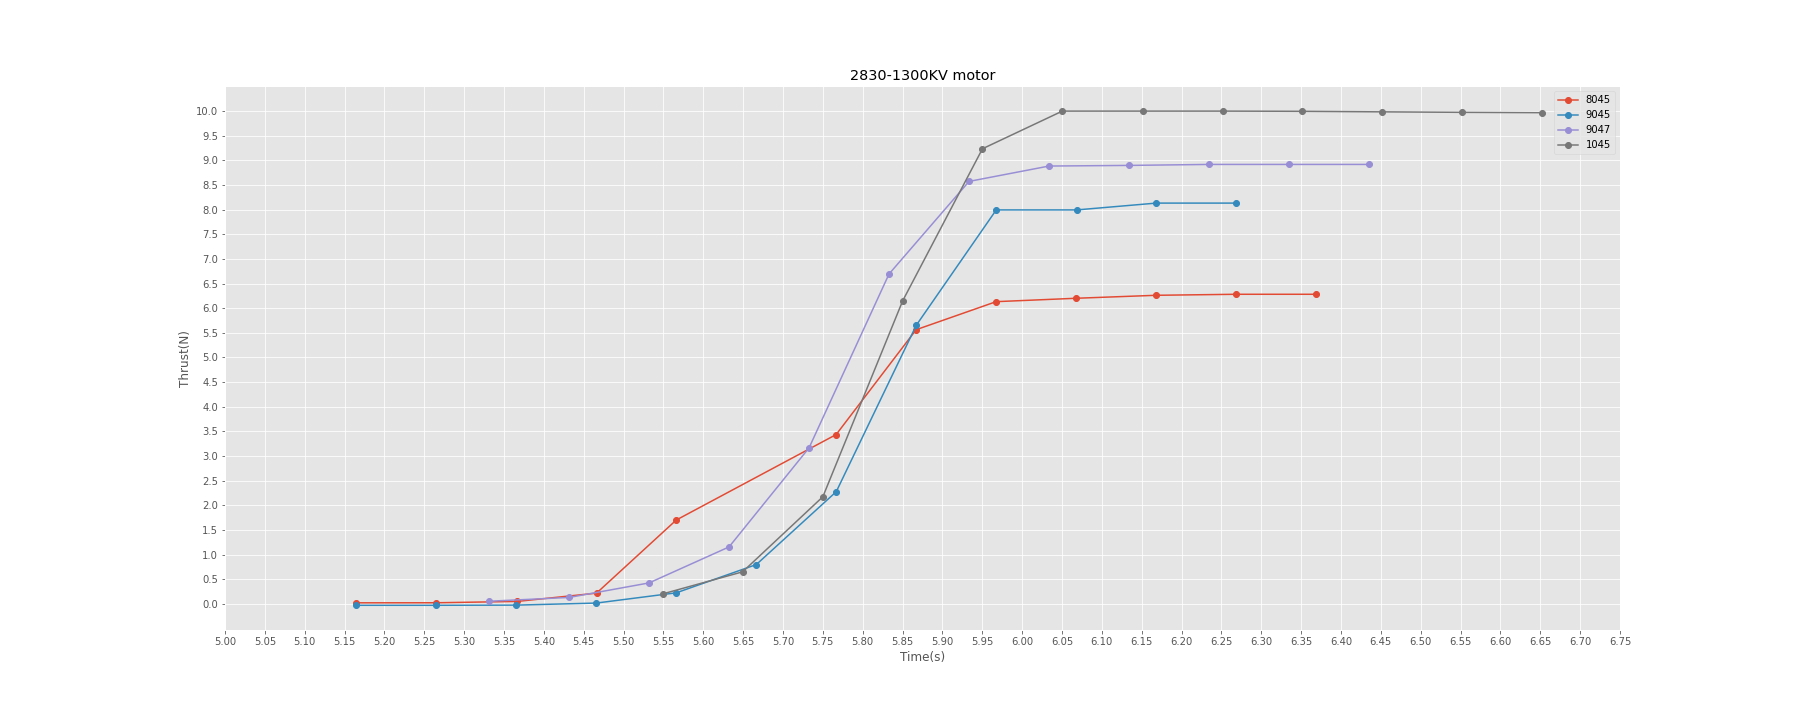
\includegraphics[width=\textwidth]{src/figs/purple_motor.png}
    \caption{1300 KV motor}
    \label{design:sts:purple}
\end{figure}
At this stage through the thrust to weight ratio analysis presented in Section \ref{thrust_analysis}, and with the current mass estimate of between 3 and 4kg, the team decided that the best choice would be to find a motor that could produce even more thrust than the  1300 KV motor in Figure \ref{design:sts:purple}. Eventually, the team found two different motors with very high torque and RPM capabilities, however they required a larger LiPo battery as well as a electronic speed controller (ESC) with a higher current rating. In the end, due to time constraints the team was not able to calibrate and test these new motors, however as will be made clear in later discussions, the setup of the electronics and software allows for motors to be "plug-and-play" and swapping out motors later on will require little to no modification to other aspects of the project. In conclusion, the team decided to move forward for now with the 1300 KV motors that were shown to produce around 10N of thrust on average.

To ensure this motor truly had to power needed, an endurance test was conducted in which the motor was throttled to 90\% for 60 seconds to determine if there was any thrust loss over time like there was with the lower torque motors. Figure \ref{design:sts:endurance} shows the results of this endurance test. Although there was some decay in thrust, the average thrust for the first 20 seconds was larger than 10N, which is presumably sufficient considering the expected mass of the rocket and flight time.
\begin{figure}[H]
    \centering
    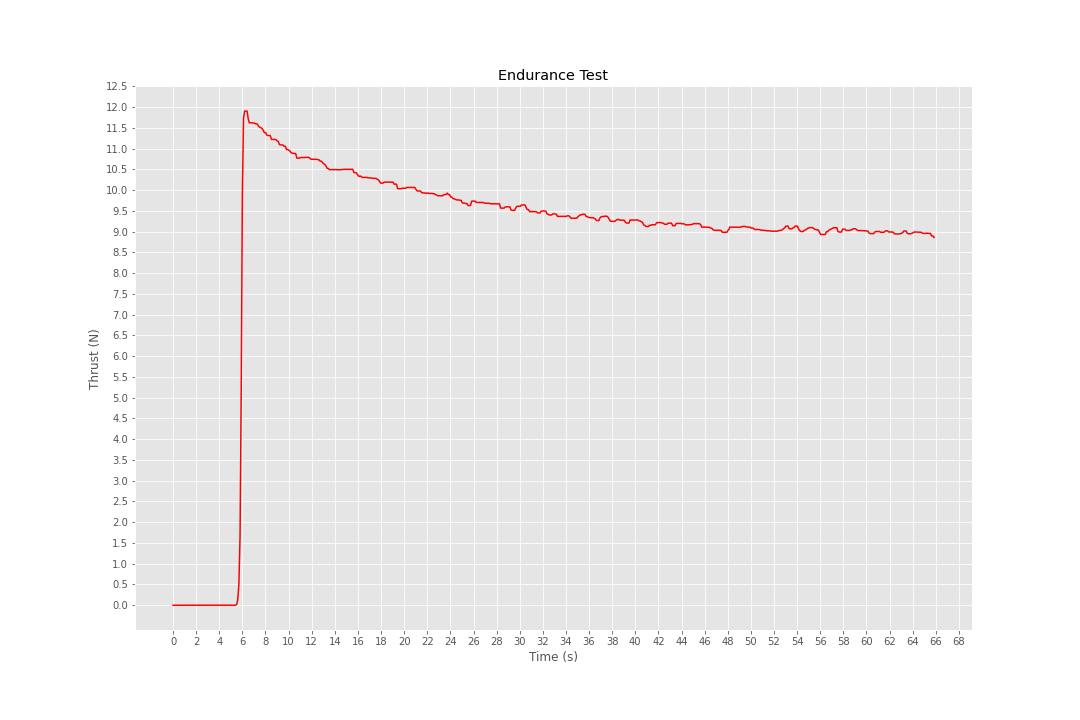
\includegraphics[width=\textwidth]{src/figs/purple_endurance.png}
    \caption{1300 KV motor endurance test}
    \label{design:sts:endurance}
\end{figure}


\section{Control System Electronics}
The onboard software and electronics are designed to detect when the rocket is falling, deploy arms and landing legs, and spin motors to enable a controlled descent and landing of the rocket autonomously without human intervention. Early on in the design and development stage of the project, the team realized that once the arms have been deployed, from an electronics and software perspective, the problem at hand is being able to autonomously "catch" and land a falling quadcopter. We operated on the assumption that the rocket being attached will make little to no difference so long as additional weight and an adjusted center of mass are accounted for. This being said, the team began by testing all electronics and software with a custom built quadcopter in parallel with the design of the rocket's arm and landing leg deployment mechanisms. This afforded the team the ability to develop each subsystem independently, and assemble components later on in a modular fashion.

\subsection{Hardware}
\label{design:controls:hardware}

\paragraph{Motors}

The voltage and current draw of the motors dictate the requirements of all other controls hardware. Quadcopters most commonly use three channel brushless DC motors due to their robustness and variety.

Brushless DC motors have fixed array of magnets on the inside of their rotor. The rotor interfaces with a stator composed of a complimentary array of wound copper wires. When a current is passed through these copper wires, an electromagnetic field capable of spinning the rotor is generated given its physical setup.

At the end of Quarter 1, we identified a promising motor candidate during testing of our STS stand. The 2830-1300 kv motor is shown in Figure \ref{fig:purple}. Note that a kv rating is equivalent to a rating of RPM per volt. Therefore, this motor is capable of spinning at roughly 14,500 RPM assuming no load attached and the use of a 3S LiPo battery. Practically speaking; however, the maximum RPM will be lower depending on the mass of the propeller. Please refer to the table below for final motor specifications.

\begin{figure}
    \centering
    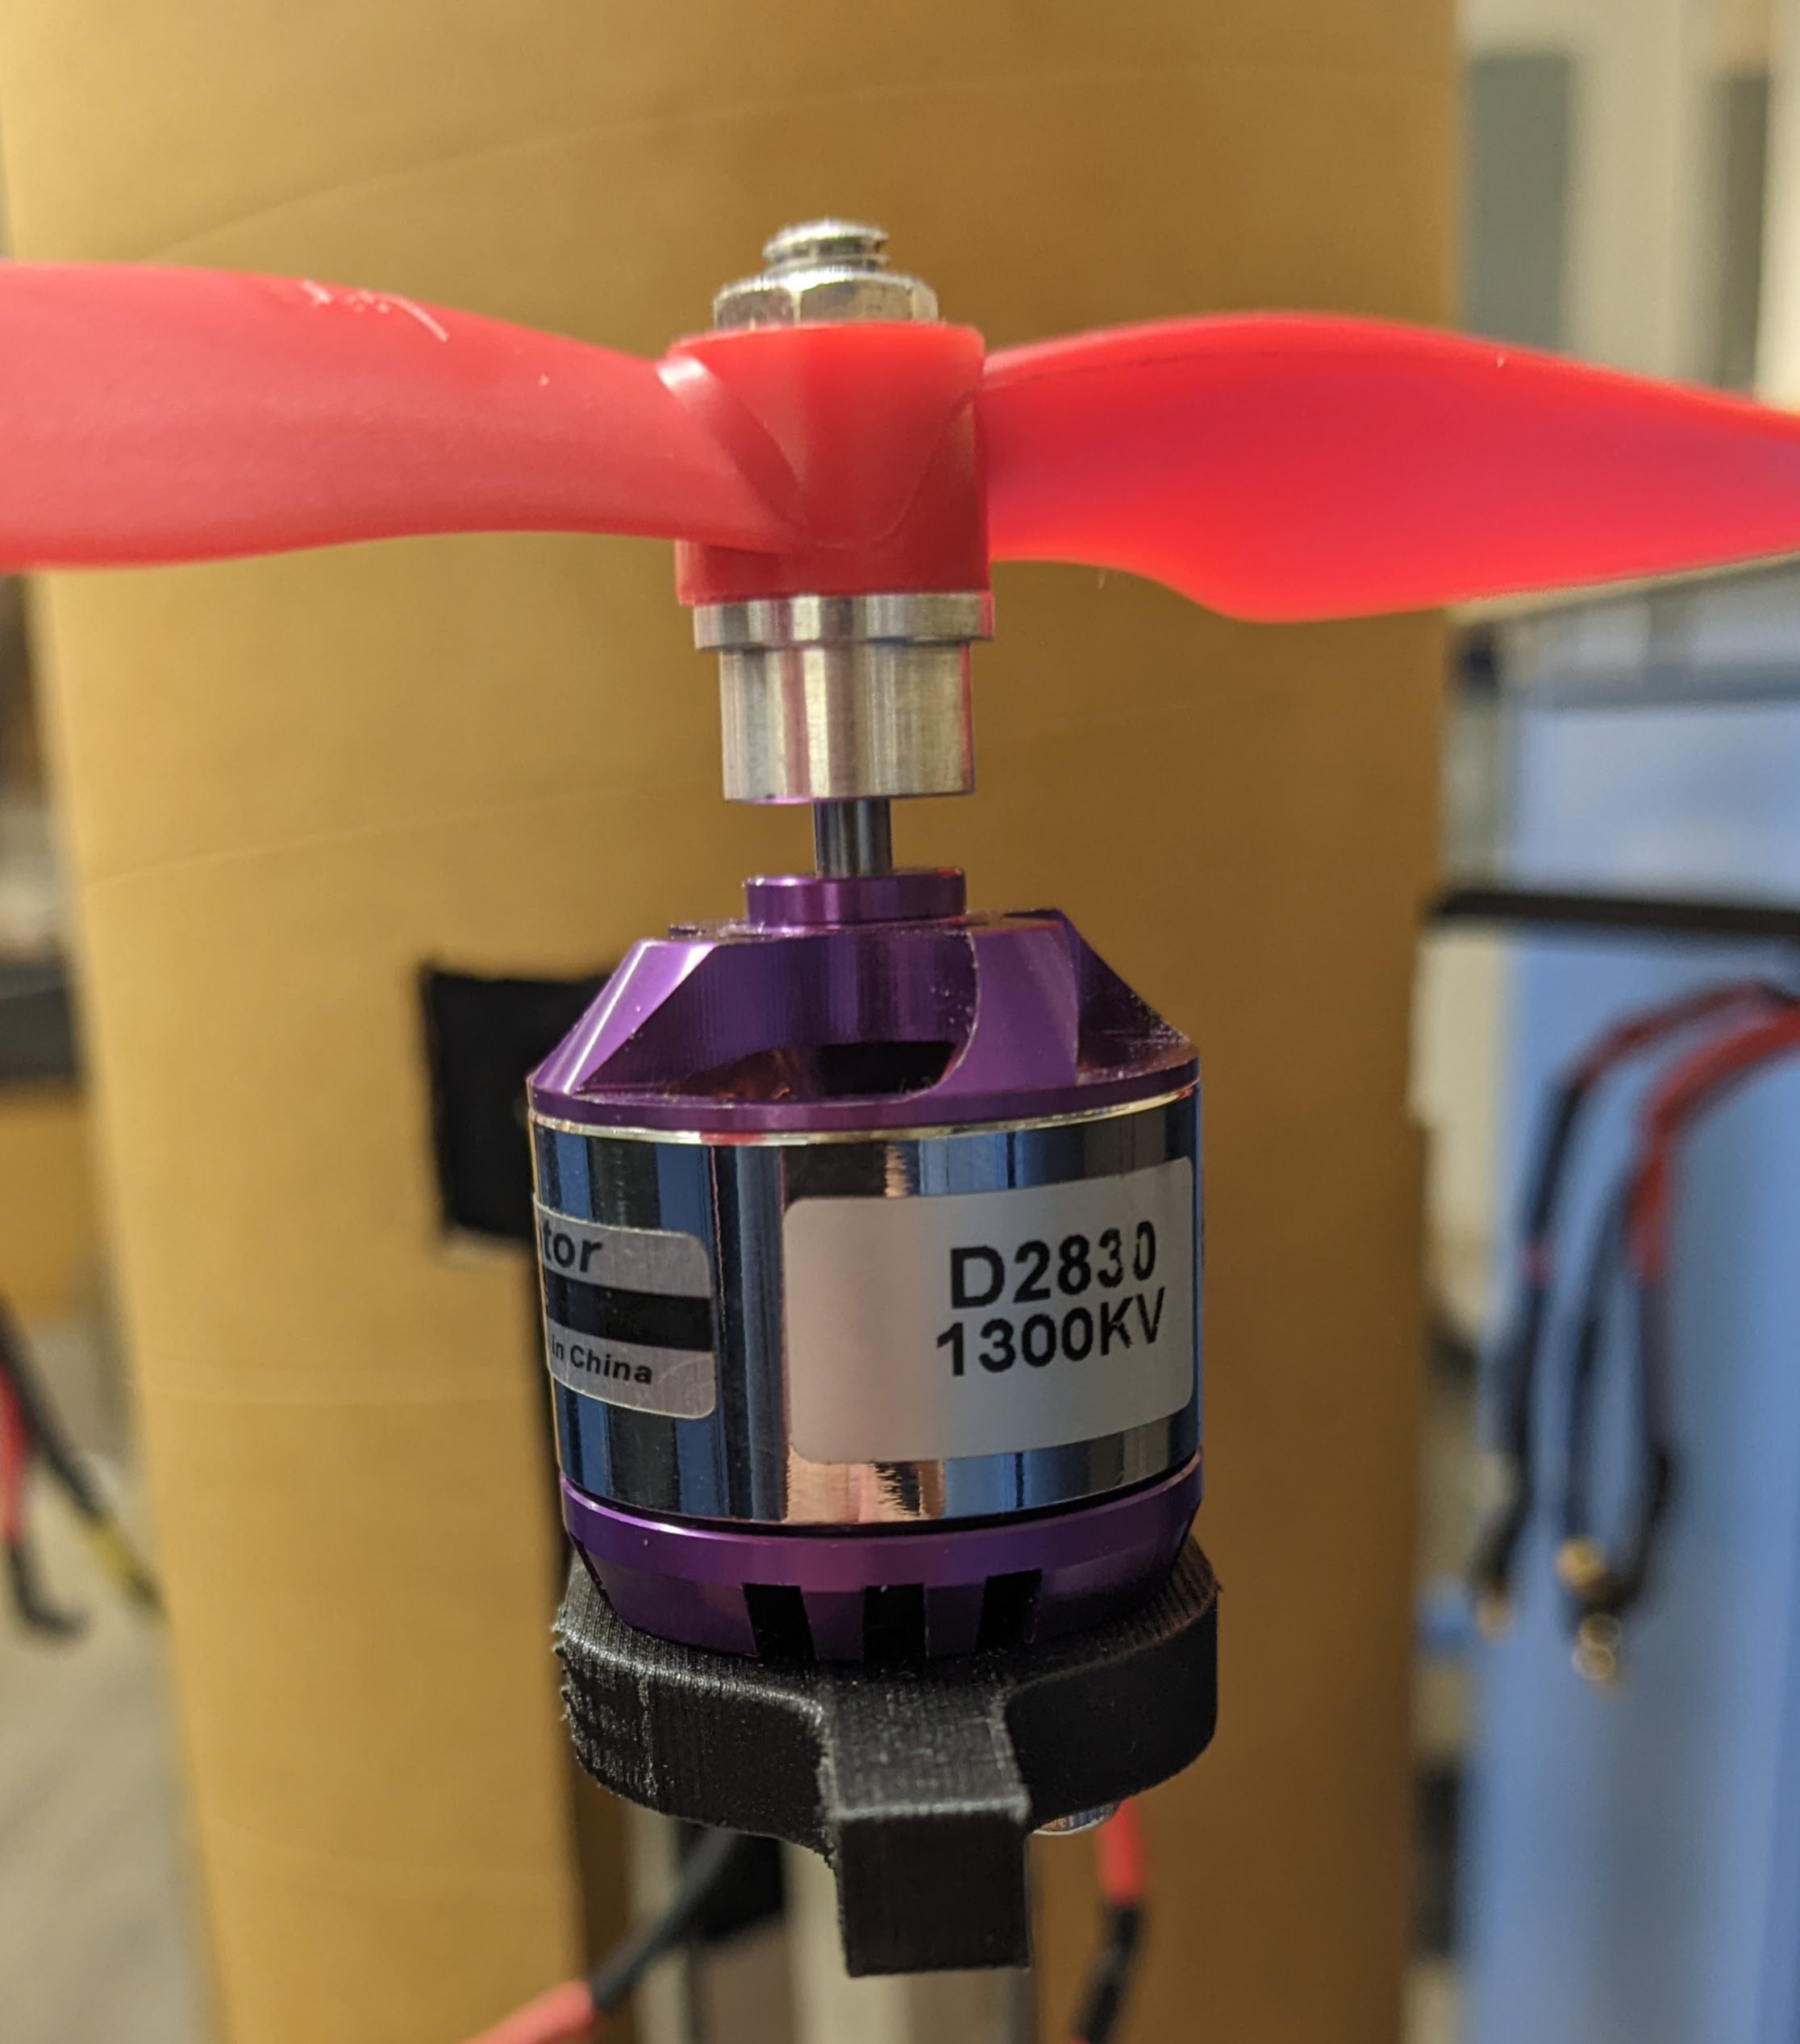
\includegraphics[scale = 0.1]{src/figs/PurpleMotors.jpg}
    \caption{Purple 1300KV motors}
    \label{fig:purple}
\end{figure}

\begin{table}[H]
\centering
% \footnotesize
\caption{Motor Specifications}
\label{design:hardware:esc-table}
\begin{tabular}{|
>{\raggedright\arraybackslash}p{.3\textwidth}|
>{\raggedright\arraybackslash}p{.2\textwidth}|
}
    \hline
     \textbf{Parameter} & \textbf{Value}
    \\\hline 
     Nominal Voltage & 7.4~15V
     \\\hline 
     Instantaneous Maximum Current (10s) & 30A
     \\\hline
     LiPo Compatibility & 2-4S 
     \\\hline
     kv & 1300
    \\\hline
\end{tabular}
\end{table}

\paragraph{Electronic Speed Controllers (ESCs)}

Using the Electronics Speed Calibrators, we are able to get extremely steady RPM of the motors with their very accurate position control. With the candidate motor selected, we were able to move onto finding an compatible ESC. There are a large variety of brushless 30A ESCs. Please refer to the table below for technical specifications of the ESC we chose.

\begin{table}[H]
\centering
% \footnotesize
\caption{ESC Specifications}
\label{design:hardware:esc-table}
\begin{tabular}{|
>{\raggedright\arraybackslash}p{.3\textwidth}|
>{\raggedright\arraybackslash}p{.2\textwidth}|
}
    \hline
     \textbf{Parameter} & \textbf{Value}
    \\\hline 
     Continuous Output Current & 30A
     \\\hline 
     Instantaneous Maximum Current (10s) & 40A
     \\\hline
     LiPo Compatibility & 2-4S 
     \\\hline
     PWM FREQUENCY & 8-18 KHz
     \\\hline
     Mass & 22 g
     \\\hline
     Dimensions & 2.17" x 1" x 0.31"
    \\\hline
\end{tabular}
\end{table}

\paragraph{Batteries}
\label{design:controls:hardware:batteries}
Lithium polymer (LiPo) batteries are by far the most common in the hobbyist drone community due to their high energy density and high discharge rate (figure \ref{fig:lipobattery}). The "S" value is the number of 3.7V (nominal) LiPo cells that are wired in series within the battery. In our case, we elected to use a 3S LiPo battery meaning that there are three 3.7V LiPo cells wired in series for a total nominal voltage of 11.1V.

\begin{figure}[H]
    \centering
    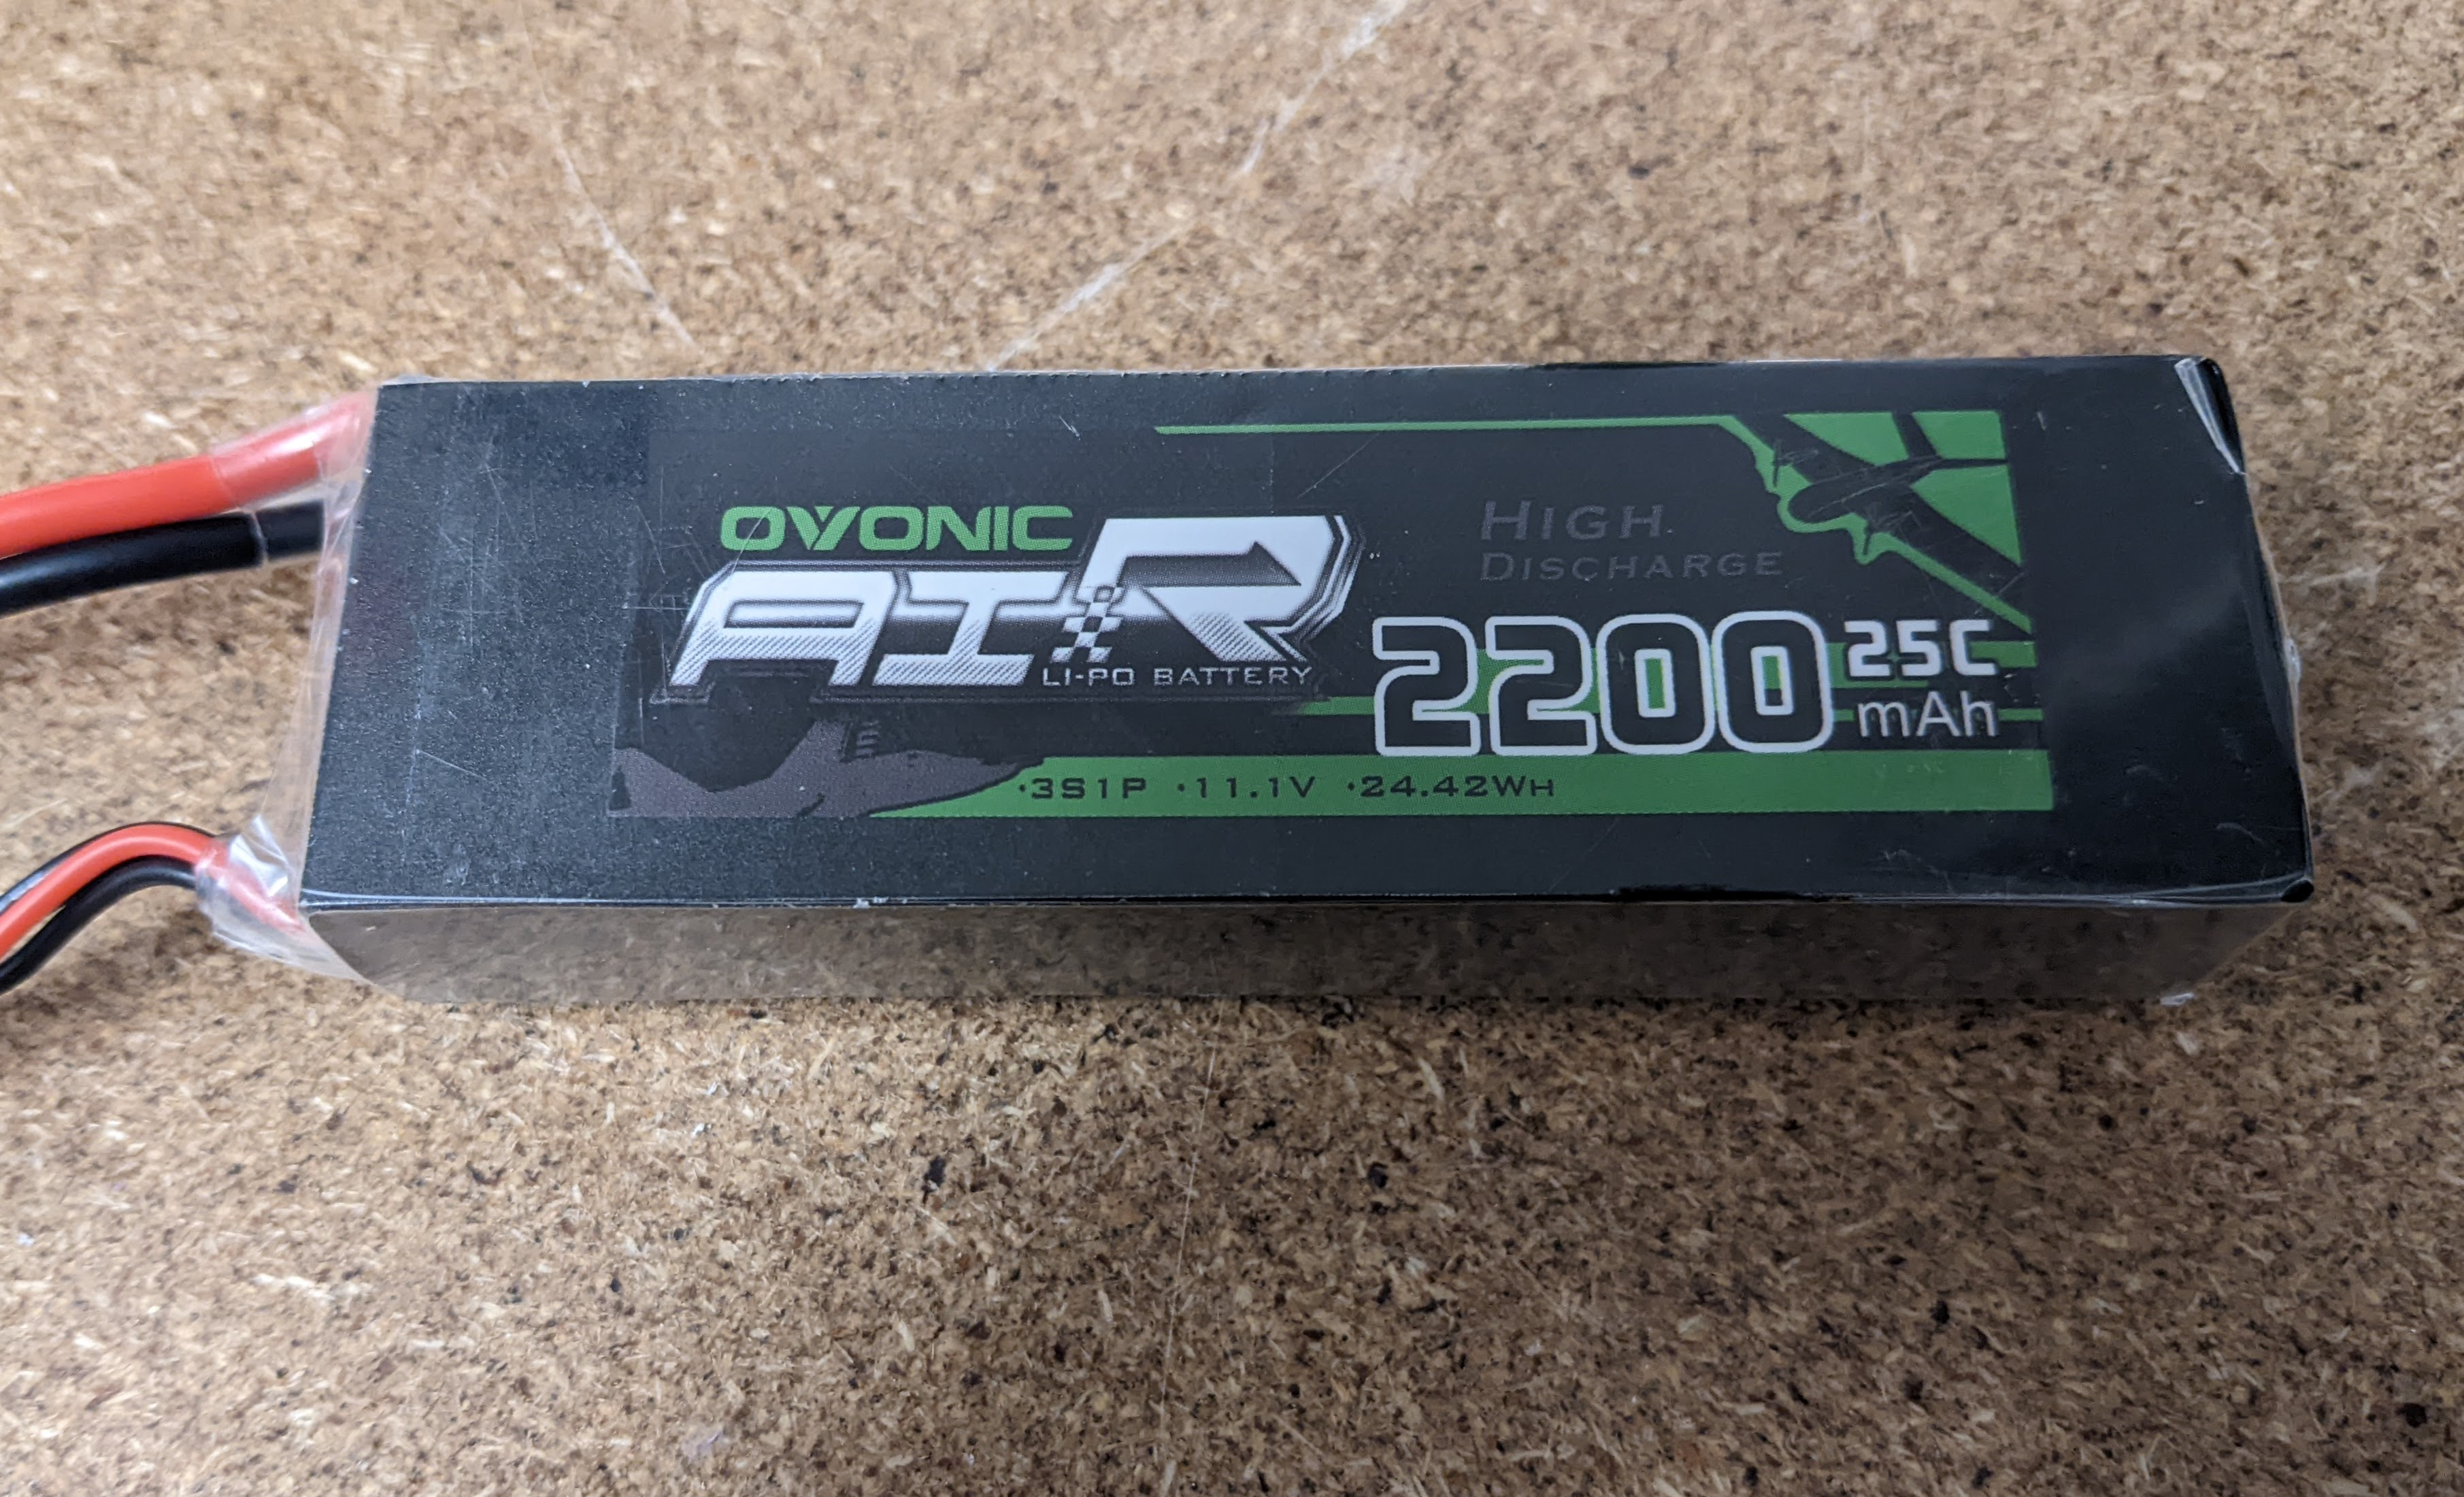
\includegraphics[width=0.5\textwidth]{src/figs/LIPOBattery.jpg}
    \caption{3-Cell Lipo Battery}
    \label{fig:lipobattery}
\end{figure}

The previous motor and ESC selections limited us to the use of 2-4S LiPo's. Choosing a 3S battery was a trivial decision as it gave us balance between increased battery mass and maximum thrust capable of being produces. Please refer to the table below for technical specifications of the battery we chose. 

\begin{table}[H]
\centering
% \footnotesize
\caption{LiPo Battery Specifications}
\label{design:hardware:esc-table}
\begin{tabular}{|
>{\raggedright\arraybackslash}p{.3\textwidth}|
>{\raggedright\arraybackslash}p{.3\textwidth}|
}
    \hline
     \textbf{Parameter} & \textbf{Value}
     \\\hline 
     Battery Type & Lithium Polymer (LiPo)
     \\\hline 
     Total Nominal Voltage & 11.1V
     \\\hline 
     Discharge Rate & 25C
     \\\hline
     Capacity & 2200 mAh
     \\\hline
     Plug & XT-60
     \\\hline
     Mass & 163 g 
     \\\hline
     Dimensions & 4.13" x 1.3" x 0.83"
    \\\hline
\end{tabular}
\end{table}

We also have a dedicated uninterrupted power supply (UPS) battery for the flight computer. UPS is important to protect sensitive electronics on computers. They function by monitoring outgoing voltage and if it dips above or below its nominal threshold, a secondary supply is called upon to return to nominal. Please refer to the table below for the technical specifications of this battery (figure \ref{fig:VGE}).

\begin{figure}[H]
    \centering
    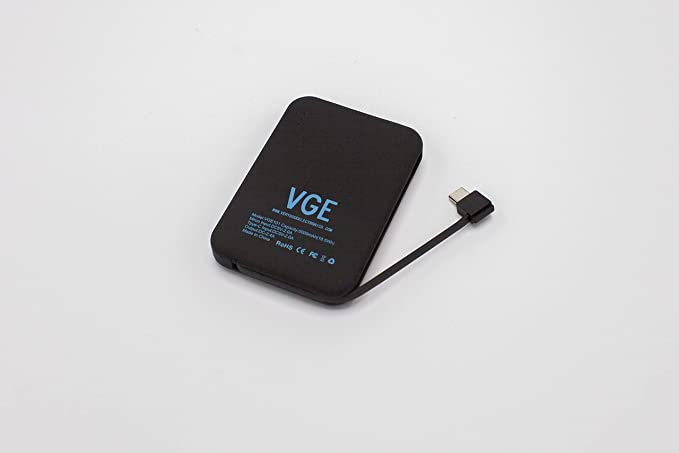
\includegraphics[width = 0.5\textwidth]{src/figs/VGE.jpg}
    \caption{Raspberry Pi Battery}
    \label{fig:VGE}
\end{figure}

\begin{table}[H]
\centering
% \footnotesize
\caption{Raspberry Pi Battery Specifications}
\label{design:hardware:esc-table}
\begin{tabular}{|
>{\raggedright\arraybackslash}p{.3\textwidth}|
>{\raggedright\arraybackslash}p{.3\textwidth}|
}
    \hline
     \textbf{Parameter} & \textbf{Value}
    \\\hline 
     Nominal Voltage & 5V
     \\\hline 
     Output Current & 2.4A
     \\\hline
     Capacity & 4000 mAh
     \\\hline
     Plug & USB-C
     \\\hline
     Mass & 142 g
     \\\hline
     Dimensions & 4.17" x 3.82" x 0.75"
    \\\hline
\end{tabular}
\end{table}

\paragraph{Power Module (PM)} 

The power module (PM) steps down LiPo battery power to 5V for the flight controller and provides full battery voltage to the power distribution board (PDB). The PM is connected to the battery via an XT-60. It feeds power to the Pixhawk via a JST connector and the other end is soldered directly to the PDB. 

\begin{figure}[H]
    \centering
    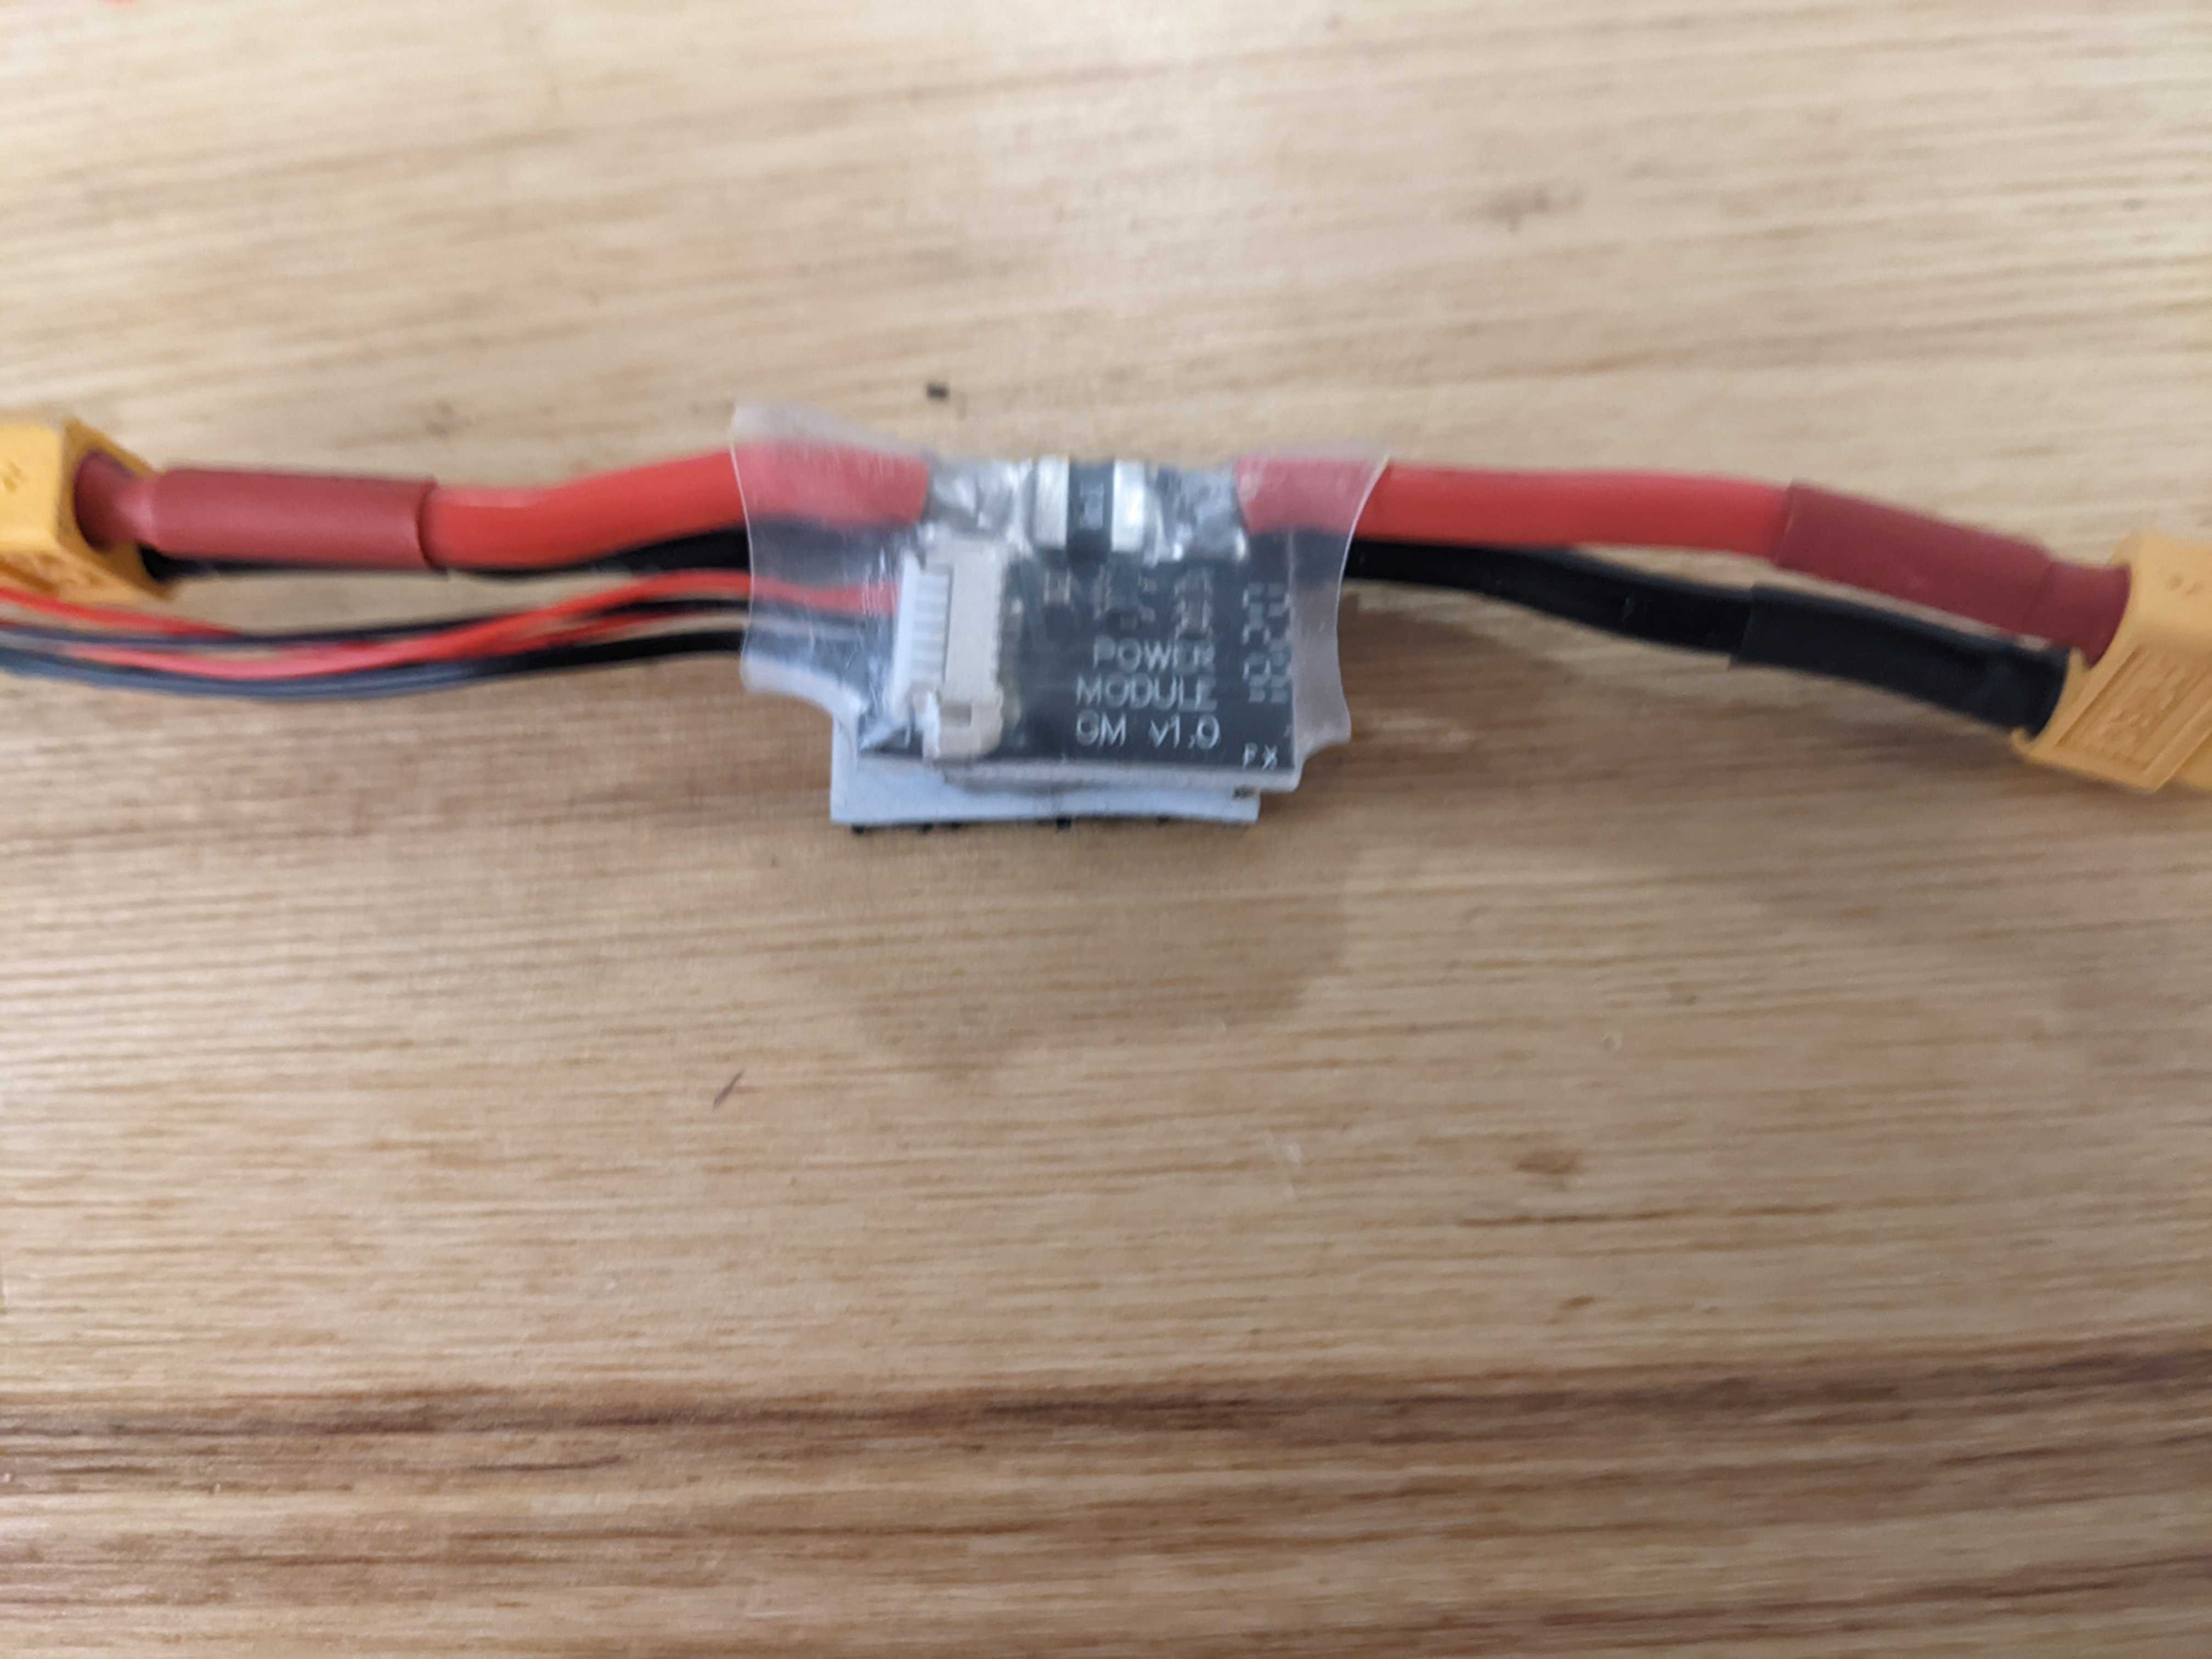
\includegraphics[width = 0.5\textwidth]{src/figs/PM.jpg}
    \caption{PM}
    \label{fig:pm}
\end{figure}


\paragraph{Power Distribution Board (PDB)}

The PDB is a rudimentary printed circuit board (PCB) whose sole purpose is to deliver the full voltage from the battery to all four ESCs without any additional logic circuitry. Copper is used due to its ability to conduct the high current present in our system. An image of ours is shown in figure \ref{fig:PDB}.

\begin{figure}[H]
    \centering
    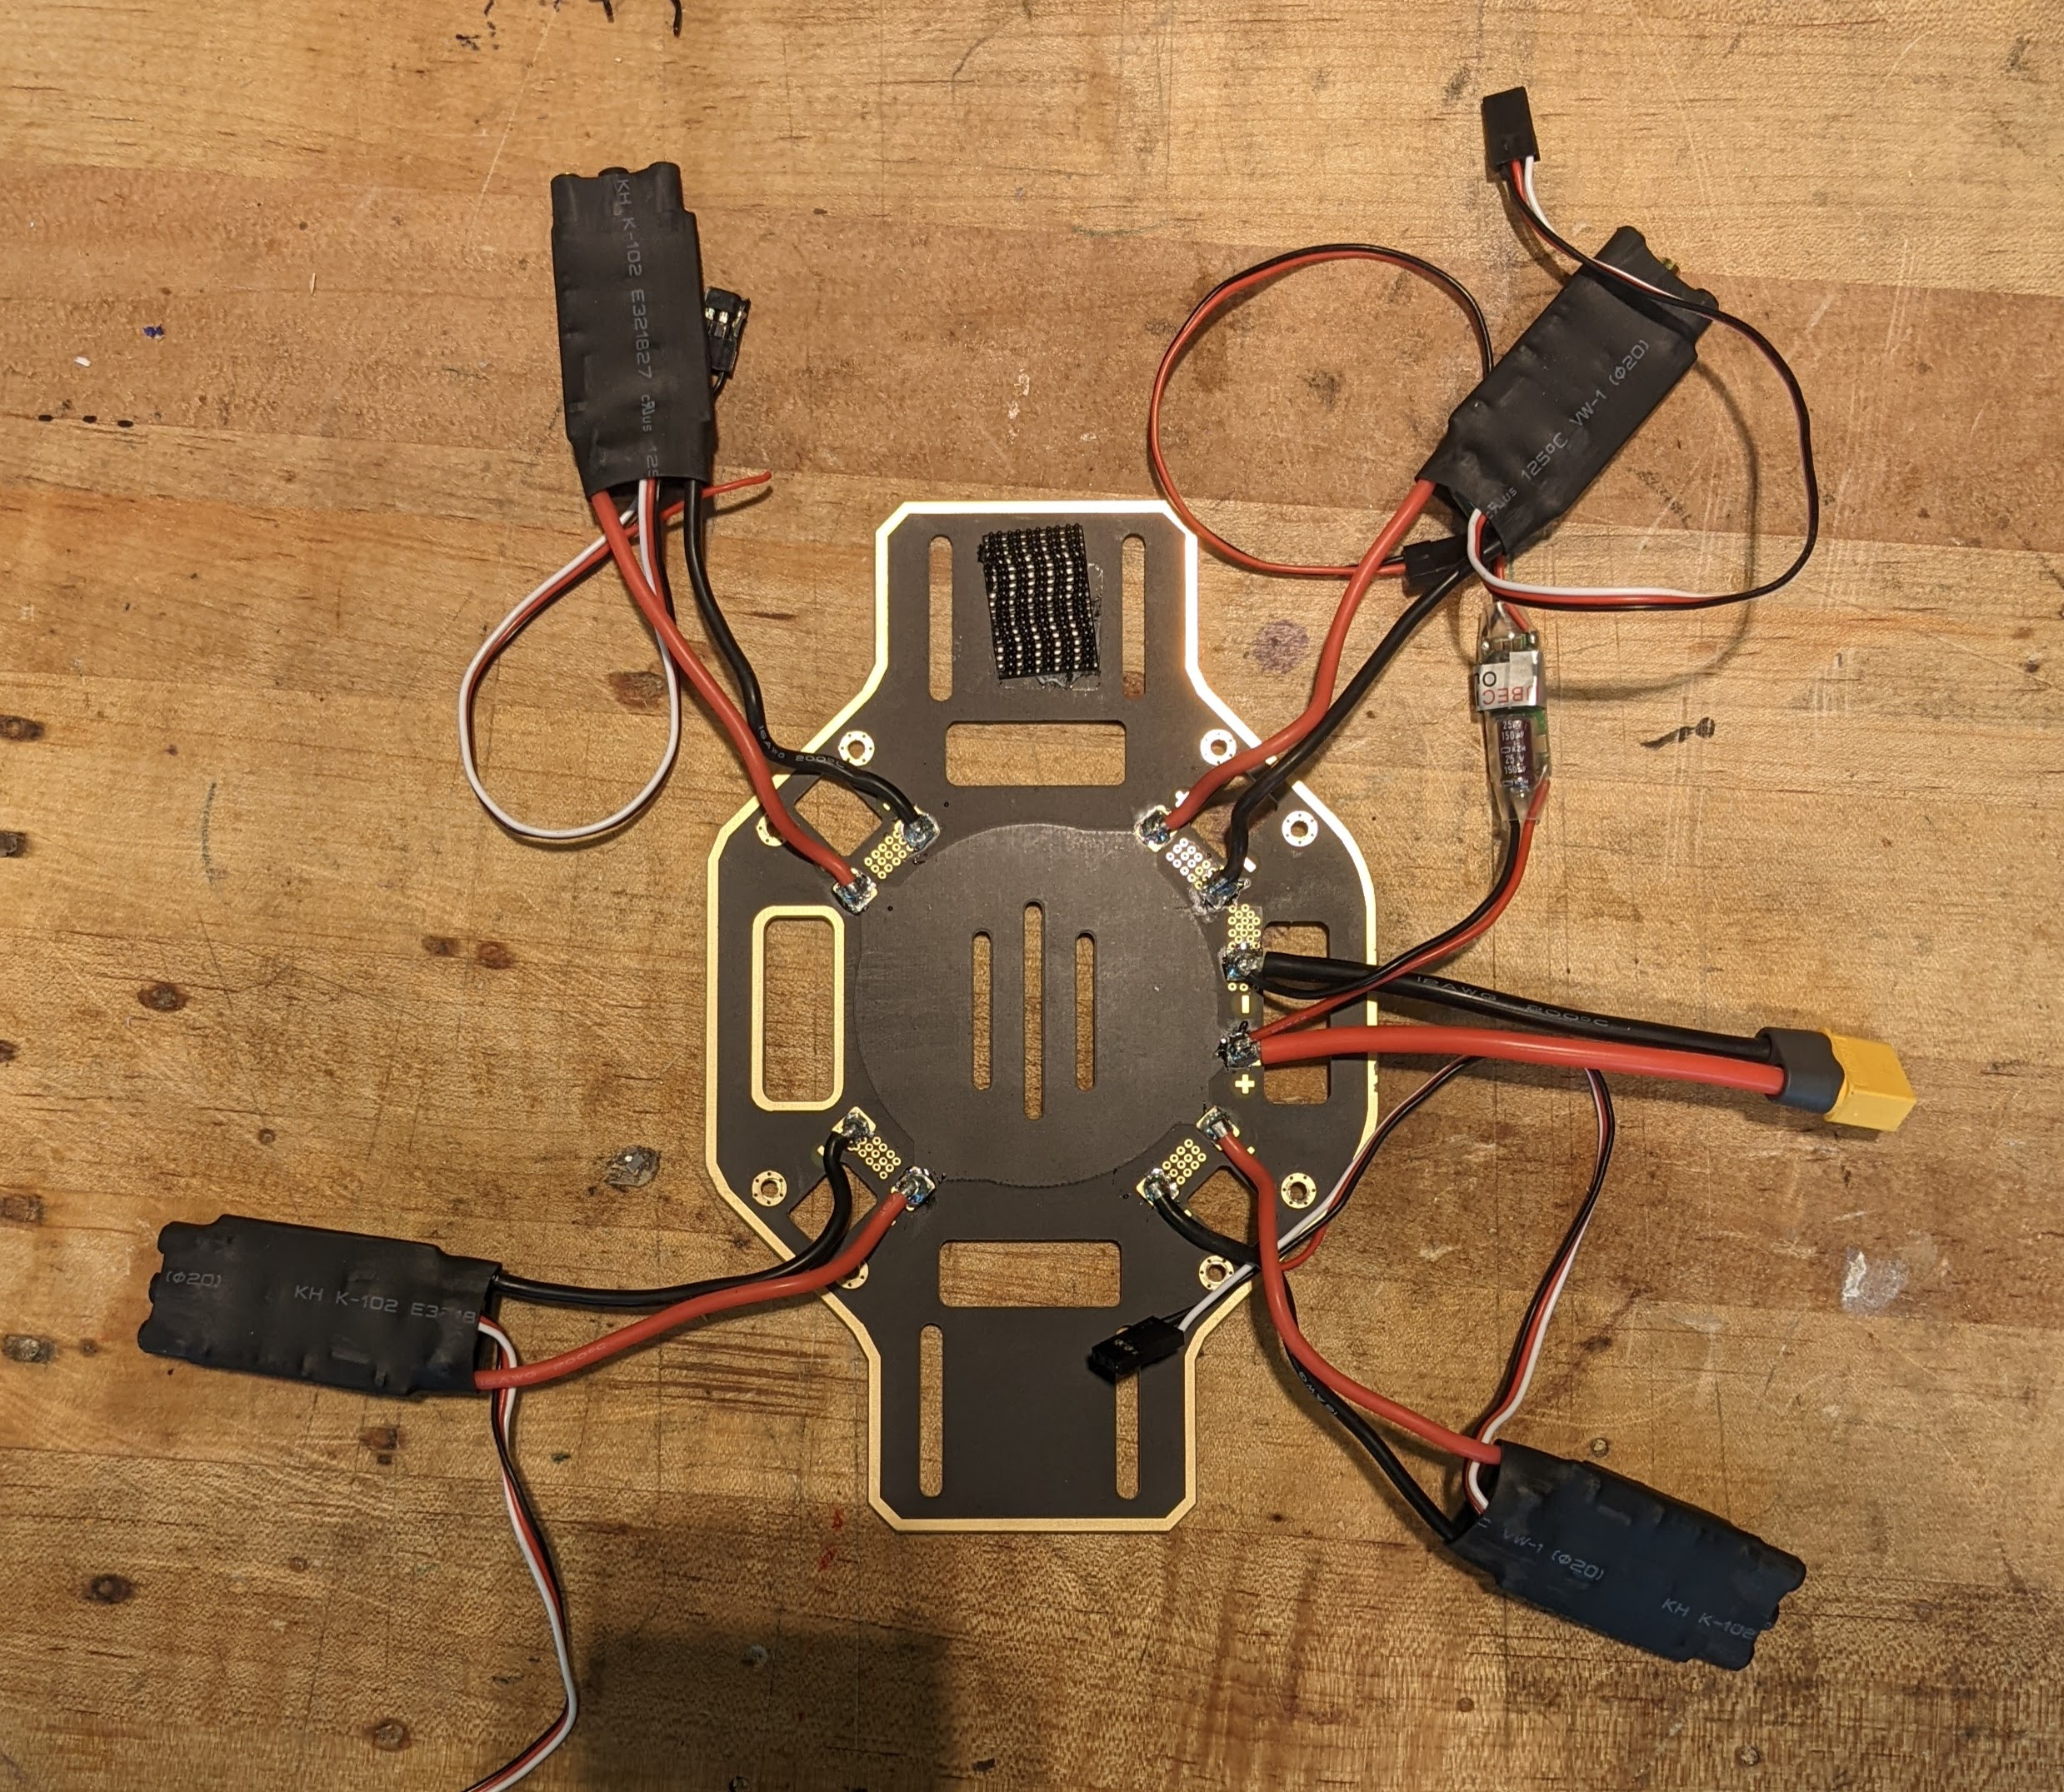
\includegraphics[width=0.8\textwidth]{src/figs/PDB.jpg}
    \caption{Power Distribution Board with ESCs}
    \label{fig:PDB}
\end{figure}

\paragraph{Flight Computer: Raspberry Pi 4 Model B}
In order to add autonomous mission capabilities, we needed an onboard flight computer. The team opted to purchase a Raspberry Pi 4 Model B as the flight computer. The Raspberry Pi was chosen since it is an inexpensive single board computer (SBC) that is commonly used for drones like the one we are building. It is designed to be easy to use for hobbyists, yet powerful enough for advanced projects. The Raspberry Pi 4B came in three different options for memory: 2GB, 4GB, or 8GB. Since the flight computer won't be running any tasks that are unusually computationally intensive, we decided we did not need the 8GB RAM model, however since the price was not that much different from the 2GB model, we opted to go with the 4GB model so we have plenty of RAM in the event that we later decide to incorporate more advanced programs. There are several useful features of the Raspberry Pi that make it a great choice for a flight computer. First, it is able to run the Linux operating system which in turn allows for us to interface with it in a very familiar and easy way. This also enables us to easily connect to the Raspberry Pi over WiFi by using SSH. Connected to the rocket during the mission with SSH is imperative since it allows us to remotely start the main program script which will be discussed later on in Section \ref{design:controls:software}.

Midway through Quarter 2 we ran into a power issue with our flight computer. We were able to SSH into it but it was not capable of sending telemetry signals to the flight controller. We noticed there were no issues when the Raspberry Pi was receiving power from an outlet and came to the conclusion that this was a power issue. We purchased a dedicated battery (See section \ref{design:controls:hardware:batteries}) for the computer and the issue was remedied. 

\paragraph{Flight Controller: Pixhawk} 
In order to control stabilization of the rocket, we decided to purchase a Pixhawk flight controller. The Pixhawk runs ArduPilot firmware and is a all encompassing "black box" solution to drone stabilization. Internal to the Pixhawk are several sensors such as an IMU and a barometer than the ArduPilot firmware uses to stabilize and fly a drone, or in this case, a rotor-powered rocket. The Pixhawk connects to the ESCs that are connected to the motors, so therefore the Pixhawk/ArduPilot is given full control over the flight dynamics of the drone/rocket. Considering the goals of the project as well as the time frame allotted to us, we decided that using the Pixhawk as a black box solution was a sound decision since programming our own stabilization software was not within the scope of the project.

\paragraph{Radio Receiver and Transmitter}
To connect to the drone via the ground station GUI, QGroundcontrol, we used an RC transmitter connected to our laptop through the USB drive. This gave us the capability to connect to a radio receiver/transmitter unit plugged into the Pixhawk flight controller through the SBus pins. This allowed us to monitor the state of the drone during flight, and calibrate all of the sensors prior to takeoff. This was critical to achieving stable flight. Additionally the handheld RC controller could connect to receiver, allowing us to fly the drone manually.

\paragraph{IMU}

The IMU is a peripheral sensor we have included to the system because we could not easily access the acceleration data being from the internal IMU on the Pixhawk. With the external IMU, we are able to read the acceleration of the rocket throughout its flight, letting us detect the drop and collect flight data. The IMU we have chosen, Adafruit BNO055 (figure \ref{fig:theIMU}), has the following specifications:

\begin{table}[H]
\centering
% \footnotesize
\caption{IMU Specifications}
\label{design:hardware:esc-table}
\begin{tabular}{|
>{\raggedright\arraybackslash}p{.3\textwidth}|
>{\raggedright\arraybackslash}p{.5\textwidth}|
}
    \hline
     \textbf{Parameter} & \textbf{Value}
    \\\hline 
     Operating Voltage & 2.4V - 3.6V 
     \\\hline 
     Digital Interface & I2C
     \\\hline
     Pull Rate & 20 Hz
     \\\hline
     Mass & 3g 
     \\\hline
     Dimensions & 0.15" x 0.2" x 1.13"
    \\\hline
\end{tabular}
\end{table}

\begin{figure}[H]
    \centering
    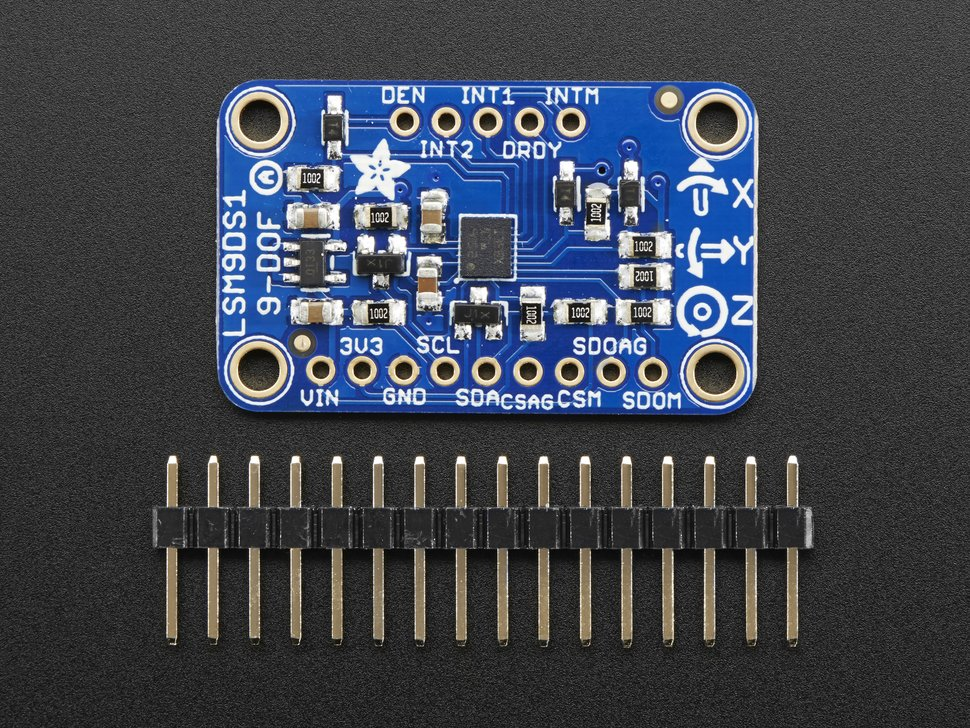
\includegraphics[width=0.5\textwidth]{src/figs/IMU_image.jpg}
    \caption{Adafruit BNO055}
    \label{fig:theIMU}
\end{figure}

\paragraph{Servo}

The arm and leg deployment mechanisms utilize a centralized 35 kg*cm torque rated servo motors, which provides the adequate torque and mount interfaces required for deployment. A servo uses high position controller with a power, ground and PWM input. Our was selected because it can be controlled via a Raspberry Pi and the position of its output spline can be precisely actuated for stowing and deployment operations. Please refer to the table below for the specifications of this motor:

\begin{table}[H]
\centering
% \footnotesize
\caption{Servo Specifications}
\label{design:hardware:esc-table}
\begin{tabular}{|
>{\raggedright\arraybackslash}p{.3\textwidth}|
>{\raggedright\arraybackslash}p{.5\textwidth}|
}
    \hline
     \textbf{Parameter} & \textbf{Value}
    \\\hline 
     Operating Voltage & 5V
     \\\hline 
     Stall Torque (at Locked) & 29 kg*cm
     \\\hline
     Stall Current (at Locked) & 1.9A
     \\\hline
     Mass & 60g
     \\\hline
     Dimensions & 1.58" x 0.79" x 1.50"
    \\\hline
\end{tabular}
\end{table}

\subsection{Software}
\label{design:controls:software}
The software to control the propulsion system is made up of two primary parts: the ArduPilot firmware running on the Pixhawk flight controller, and the Python DroneKit scripts running on the Raspberry Pi flight computer. \href{https://github.com/ArduPilot/ardupilot}{ArduPilot} is an open source autopilot software for drones and other similar vehicles and it is very reputable and well maintained. The DroneKit Python library which is used on the Raspberry Pi flight computer to program autonomous missions is very commonly used in the hobby drone world and offers an easy to use front end for sending MAVLink messages to ArduPilot.

\paragraph{Ardupilot}
As mentioned in Section \ref{design:controls:hardware}, the stabilization and control software used in this project uses several "black box" solutions, and ArduPilot is one of them. ArduPilot, although customizable, handles stabilization and flight dynamics under the hood. It works by taking data from an onboard inertial measurement unit (IMU), and uses a series of feedback loops to control the orientation of the vehicle (in this case quadcopter/rocket).
Considering the time frame and goals, the team decided that developing any form of custom stabilization, flight, or control software outside of ArduPilot was beyond the scope of the project, and ArduPilot was used on the Pixhawk without modification other than basic settings such as number of propellers, 

\paragraph{Scripting Functionality}
The goal of the Python script running on the Raspberry Pi is to interface with an external IMU, as well as the Pixhawk to determine when the rocket is falling, trigger arm and landing leg deployment, and control the rotors to bring the rocket to a hover and land. The main program loop for this code can be found in Appendix \ref{app:main-code} as well as on GitHub: \url{https://github.com/nmarks99/aero-capstone}. 

For reading data from the external IMU connected to the Raspberry Pi over I2C, a Python library from Adafruit's CircuitPython is utilized. In order to ensure consistent readings that do not interfere with the main program loop, the team decided to read IMU data in a separate thread using Python's threading module. Before the main program loop begins, a separate thread is started and from then on, data is read from the IMU concurrently with the main program. To share this data with the main program loop, the IMU data is saved into a mutable array (Python list) that is updated with new IMU values as they are received. At the start of the main loop, the last (most recent) value in the array of IMU data is checked to see if the acceleration is above a threshold value. 

Once drop has been detected, a MAVlink command is sent to the Pixhawk over UART to spin the arm and leg deployment servo using the pymavlink module within the DroneKit library. At this stage, arms and legs are deployed and now the rocket can begin attempting to slow itself down and bring itself to a hover. This is done by setting sending a MAVLink commmand to set the thrust to a maximum value and the thrust will be held at a maximum until the IMU reads that the rocket has reached a hover again. Finally, once hover has been reached, using DroneKit, the vehicle will be set to land mode which will automatically land the rocket below wherever it is hovering at.


\section{Propulsion Arm System}
Of the three main systems that make up the full prototype, the propulsion arm system which underwent the most iterative design process. The Propulsion Arm System development in Quarter 2 was kickstarted by the Quarter 1 Arm Deployment Test Stand (ADTS). The current system is composed of similar components to the ADTS as well as a variety of smaller components that took a rudimentary prototype to a fully functional and reliable system.
\subsection{Propulsion Arms}
The original arms from Quarter 1 on the arm deployment test stand were designed to support a 5" propeller blade. The deployment springs were attached by inserting their legs into two holes drilled into the back of the arm. The arm deployment test stand with the arm attached to it via springs is shown in figure \ref{fig:adts}. Since this initial design the arm has undergone 14 total iterations and 3 significant design changes. 

\begin{figure}
    \centering
    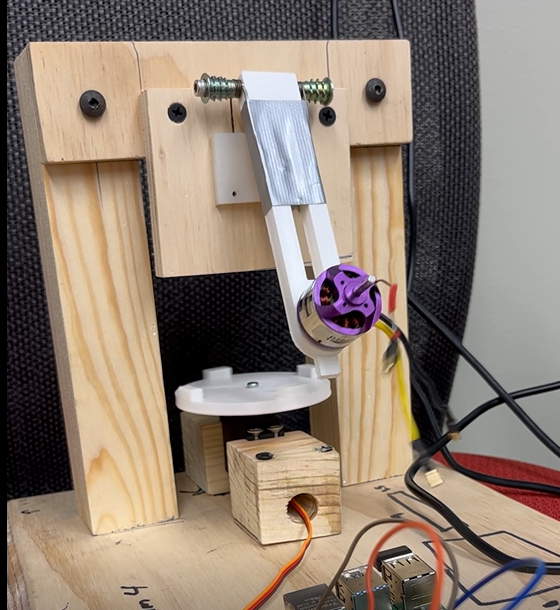
\includegraphics[width=0.5\textwidth]{src/figs/ADTS.png}
    \caption{Original Arm Deployment Test Stand}
    \label{fig:adts}
\end{figure}

In the start of Quarter 2, the team realized that the product would require substantially larger blades than originally planned for. Design of a new arm capable of supporting an 8" propeller blade began and within a week an arm that could be attached to the arm core and support an 8" blade had been modeled and printed. The team worked with this arm size for the majority of the quarter with minor changes occurring including adding 'speed holes' to reduce drag and weight (see figure \ref{fig:speedholes}), reducing arm thickness to reduce mass, and adding ribs along the length of the arm to increase bending strength (see figure \ref{fig:speedholes}). Testing of this arm mainly involved securing 4 of them to the core and working on deployment tests using the pre-deployment locking mechanism and torsion springs. It was found that the arm deployed quickly but once deployed it had the ability to both slide side to side in the bay but also twist. It was determined that this was a result of using bolts that did not provide a tight enough fit between the arm and core.

\begin{figure}
    \centering
    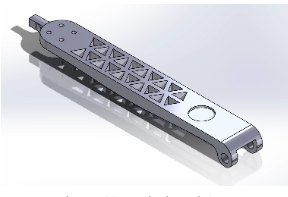
\includegraphics[width=0.5\textwidth]{src/figs/armwithspeed.png}
    \caption{Speed Holes on arm}
    \label{fig:speedholes}
\end{figure}

The second serious design change came when the team realized that 8" blades would no longer provide the thrust needed to support our platform. This realization came with a redesign of the arm to support 10" blades. This involved lengthening the arm as well as performing a new ANSYS simulation to ensure that the arm would still be able to withstand the moment caused by the thrust. This arm was attached to the core for testing using 1/4" shoulder bolts as opposed to the M6 bolts found in the Ford Prototyping Shop and to further prevent side to side motion, the core end of the arm was widened to reduce total clearance with the bay walls from 0.15" to 0.05". These two changes proved successful in better securing the arm and eliminating twist according to observations made.

The third and final serious design change came with the final selection of the motor and propellers that are used on the alpha prototype. The larger, 2830 stator size motors were significantly taller than the previous motors that were used for testing. To allow these motors to still fit within the diameter of the 6" rocket body, a 5/8" step-back was added to the arm. This allowed the core to remain unchanged while allowing all components to fit inside the rocket body. The final arm can be seen in figure \ref{fig:newarm}.

\begin{figure}
    \centering
    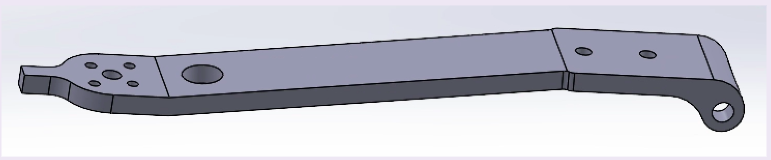
\includegraphics[width=0.75\textwidth]{src/figs/finalarm.png}
    \caption{Final Arm Design}
    \label{fig:newarm}
\end{figure}

The stepped-back arm design is the propulsion arm currently in place on the alpha prototype. This arm is capable of supporting blades up to 10" in diameter, allowing for 1/2" clearance from the rocket body when fully deployed. This arm mounts to the central core, discussed in coming sections using a 1/4" shoulder bolt that passes through it on the underside as well as through both bay walls on the core. Additionally, the arm is capable of supporting any motor that has a 16mm x 19mm mounting pattern that is less than 2" in total height with a mounted propeller. It was critical that the propulsion arm was incredibly stiff since it would be undergoing the largest loading of any component in the entire prototype. To get a component this stiff while keeping it as light as possible, it was 3D printed using Onyx with carbon fiber inlay. This material has the bending stiffness of 6060 T6 Aluminum, and when modeled in ANSYS, the arm deflected less that 1 millimeter under loading with a 1.5 Factor of Safety. For more information on this ANSYS simulation, please see section \ref{propulsionarmansys}. In addition to the motor mount, the final propulsion arm also incorporates the following features.

\begin{itemize}
    \item Pre-Deployment Locking Mechanism Interface Tab
    \item Through Hole to allow motor wires to pass to underside of arm
    \item (2) countersunk M3 screw holes for deployed locking mechanism attachment
    \item (2) shoulder bolt supports for attachment to the core
    \item (2) torsion spring alignment slots
\end{itemize}

\subsection{Deployment Method}
In Quarter 1, the team researched propulsion arm deployment methods. The most defining requirement for the arm deployment mechanism was that it was quick to prevent the rocket from gaining too much velocity and impacting the ground before it could be slowed. A variety of options were researched including a geared system, servos, hydraulic springs, and torsion springs. The geared system and hydraulic springs were eventually eliminated from the selection process as both would either be too heavy or too complex to implement in a small scale, amateur rocket. Of the remaining two contenders, the servos were explored first. The team purchased two servos that were believed to have a torque sufficient to lift our initial arm prototype 90 degrees. It was found that the smaller of the two servos was not only too slow, but also not strong enough to fully lift the arm, which was 1/4 the size of our alpha prototype arm. After this test, the team decided to move away from the use of four servos in an effort to minimize weight and power requirements. With servos now eliminated, torsion springs were the leading concept. Several springs of varying spring constants were purchased and tested. Due to their quick, reliable, and simple nature, torsion springs were selected as our final propulsion arm deployment method. Initially, the team was using 2, 90 degree torsion springs on each arm. One left hand wound and one right hand wound spring on each arm. However, it was found that despite having a 90 degree free angle, their range of use before plastic deformation was limited to about 60 degrees of compression. As a result of this discovery, the team switched to using 120 degree torsion springs. Double torsion springs were briefly looked into but it was found that no double torsion springs that were narrow enough to fit under the arm would provide a spring constant high enough to fully deploy the arm. As previously stated, the team decided to use two, 120 degree torsion springs on each arm. This would allow the spring to compress 90 degrees while staying in its elastic deformation regime. The selected springs are for a 0.296" shaft and have a maximum torque of 3.54 in-lbs at their fully compressed position.


\paragraph{Pre-Deployment Locking Mechanism}
\label{pre-deployment_arm}
To complement the selection of torsion springs as the propulsion arm deployment method, a mechanism that blocked the arms' path of travel would be required since the torsional springs cause the arm to naturally want to deploy. In effort to reduce mass, the team wanted to proceed with a mechanism that worked for all four arms simultaneously as opposed to having a mechanism for each arm. The team came up with two leading ideas, each of which involved an 'unlocking disk' that was actuated through the use of a single servo. The first design latched with four doors that would be situated on the outside of each arm bay. Inside the rocket, the torsion springs would be pushing the arm against the inner face of the door. When rotated, the disk would unlatch the door allowing the arms to push the door open and fully deploy. The second idea followed similar suit but instead, latched the arms inside the rocket as opposed to the latching doors. It did this by being situated below the stowed arms and having four tabs that stuck vertically out of its surface. These tabs were at a diameter so that when the arms were vertically stowed, the tabs would interface with the end of the arm, blocking their travel. Design idea \#1 was selected by the team to proceed with since it combined two functions, securing the bay doors, and securing the arms. A CAD model was quickly made so the idea could be demonstrated to the professors in our next meeting. These can be seen in figure \ref{fig:diskdoor} and \ref{fig:doorlatch}. However, in that meeting with the Capstone Professors, they advised us that designing a system that combined the two functions was too ambitious and instead heavily recommended that we proceed with design idea \#2. This idea was then completely redone in SolidWorks to begin printing and testing.

\begin{figure}[H]
    \centering
    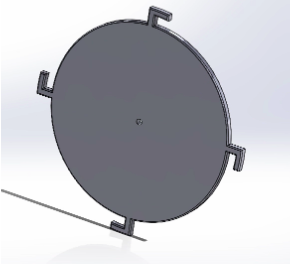
\includegraphics[width=0.5\textwidth]{src/figs/doordisk.png}
    \caption{Final Arm Design}
    \label{fig:diskdoor}
\end{figure}
\begin{figure}[H]
    \centering
    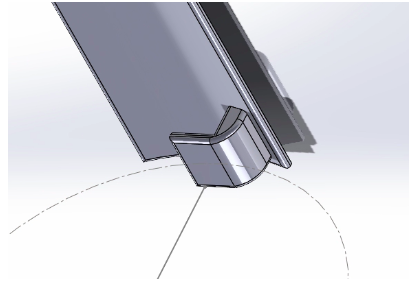
\includegraphics[width=0.5\textwidth]{src/figs/doorlatch.png}
    \caption{Final Arm Design}
    \label{fig:doorlatch}
\end{figure}

Quarter 1 ended with the team having a functional propulsion arm deployment system involving a small arm, 2 torsion springs, and an unlocking disk mounted below the stowed arms which spun when a servo was commanded to rotate. The quarter one prototype, also known as the Arm Deployment Test Stand (ADTS), can be seen in figure \ref{fig:adts}.


Since this initial Quarter 1 prototype, design of the pre-deployment locking disk has remained nearly the same. Changes were made to the diameter of the disk and the positioning of the tabs in accordance with changes to arm thickness and position within the rocket body. These changes were only a matter of redefining dimensions in the SolidWorks part and reprinting. The first real change came late in Quarter 2 after increasing the torsion springs spring constant. With the added torque from the springs, the team noticed during testing that the servo was spinning but the disk was not. It was found that this was a result of the M3 fastener that secures the disk to the servo slipping from the added torque. To remedy this problem, one of the provided attachments for the servo was attached and a small extruded rectangular cut was made in the bottom of the disk. This allows for the servo attachment to rotate with the servo, preventing slipping. This cutout can be seen in figure \ref{fig:cutout} This change completely fixed the problem and the design of the unlocking disk did not change until just before the alpha prototype. 

\begin{figure}[H]
    \centering
    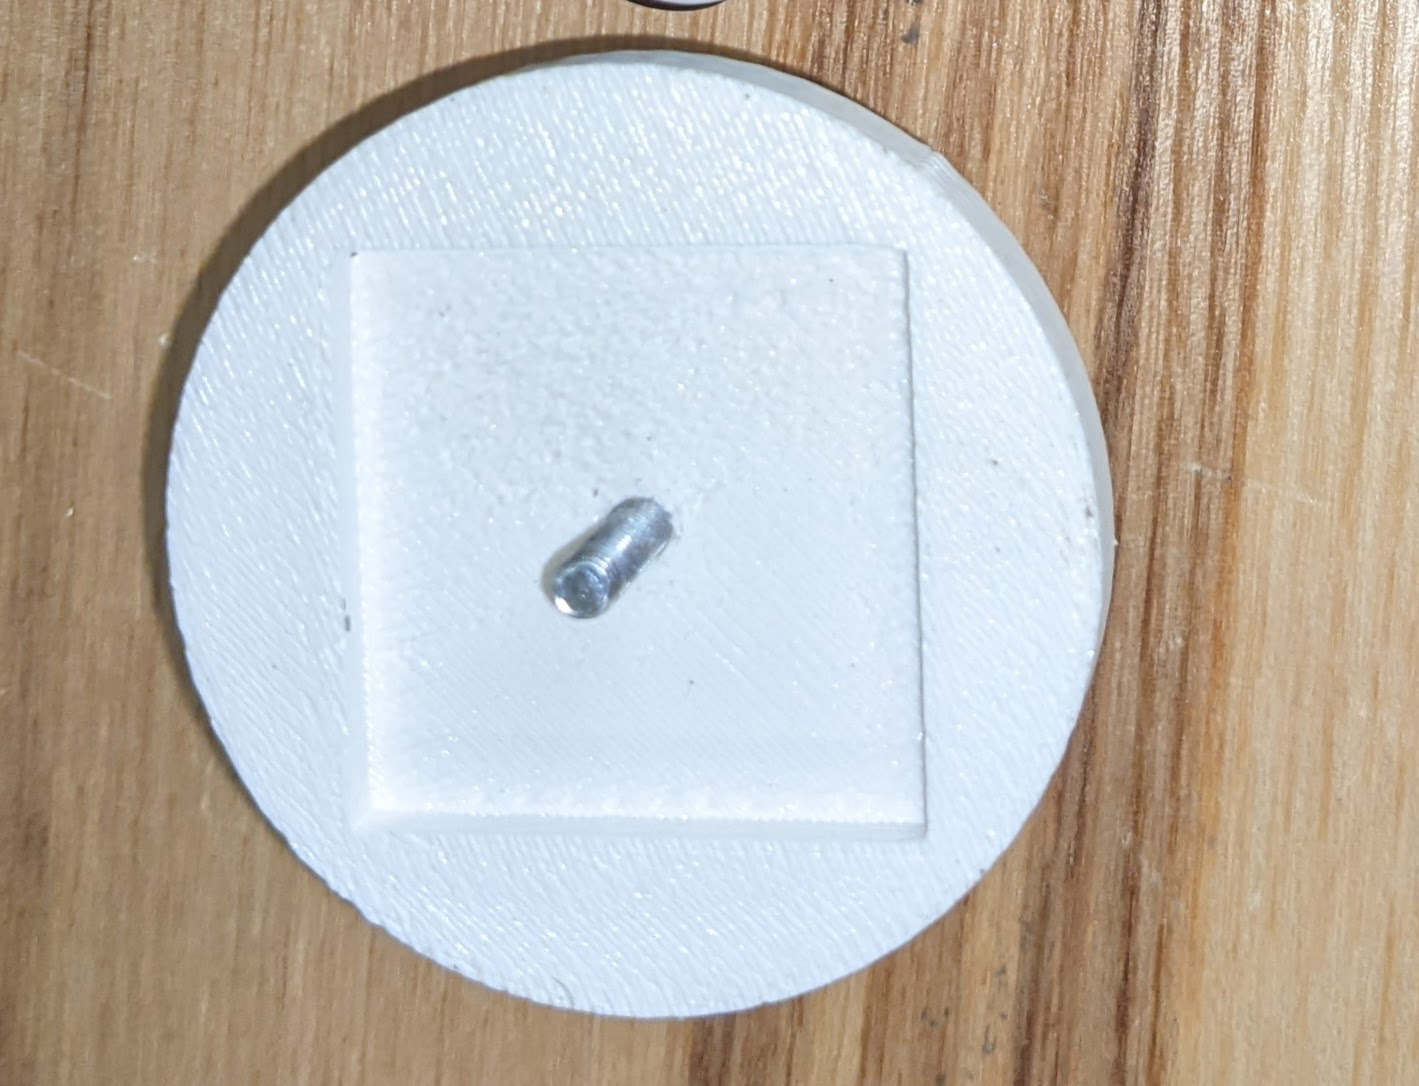
\includegraphics[width=0.5\textwidth]{src/figs/Spool_Cutout.jpg}
    \caption{Cutout to Prevent slipping}
    \label{fig:cutout}
\end{figure}

With the end of the quarter approaching and the entire alpha prototype designed and built, the team began a tedious process of mass reduction. In this process, it was found that both the legs and arms could be deployed simultaneously. Previously, one servo was used for arm deployment, and one was used for leg deployment (more on this in following sections). In order to reduce mass, the team elected to combine these functions and instead use one servo for both arm and leg deployment. To accommodate this change, a long stem was added to the bottom of the pre-deployment locking disk, this allowed it to nest with the leg pre-deployment locking mechanism, discussed later. They nest via a 0.25" hole in the bottom of the disk stem using M2 threaded inserts and screws. Concurrent with this change, the diameter was changed one final time to accommodate the alpha propulsion arms which involved the step-back design which greatly reduced the size of the disk (1.25" diameter reduction). This design is present in the alpha prototype and is 3D printed using ABS. Figure \ref{fig:extendeddisk} shows the extended disk. Figure \ref{fig:combined attachments} shows the two combined pieces. 

\begin{figure}[H]
    \centering
    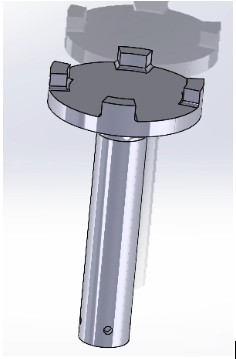
\includegraphics[width=0.3\textwidth]{src/figs/extendeddisk.png}
    \caption{Extended Disk}
    \label{fig:extendeddisk}
\end{figure}

\begin{figure}[H]
    \centering
    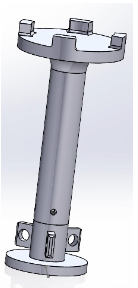
\includegraphics[width=0.2\textwidth]{src/figs/combinedattach.png}
    \caption{Combined Servo Attachments}
    \label{fig:combined attachments}
\end{figure}

\paragraph{Servo Holder}
To secure the servo for arm deployment in place, the team designed a servo holder (figure \ref{fig:SH}). This holder was a single piece that slid over the inner rails of the support structures (discussed in following sections). It had a box that provided a tight fit with the servo in the center of it that would allow the spindle of the servo to be perfectly centered in the rocket. This design was printed out of ABS and worked well for testing. However, it was later combined with another component during the mass saving process and does not present itself in the alpha prototype. This combination will be discussed in the section detailing the design of the inner assembly support plates.

\begin{figure}[H]
    \centering
    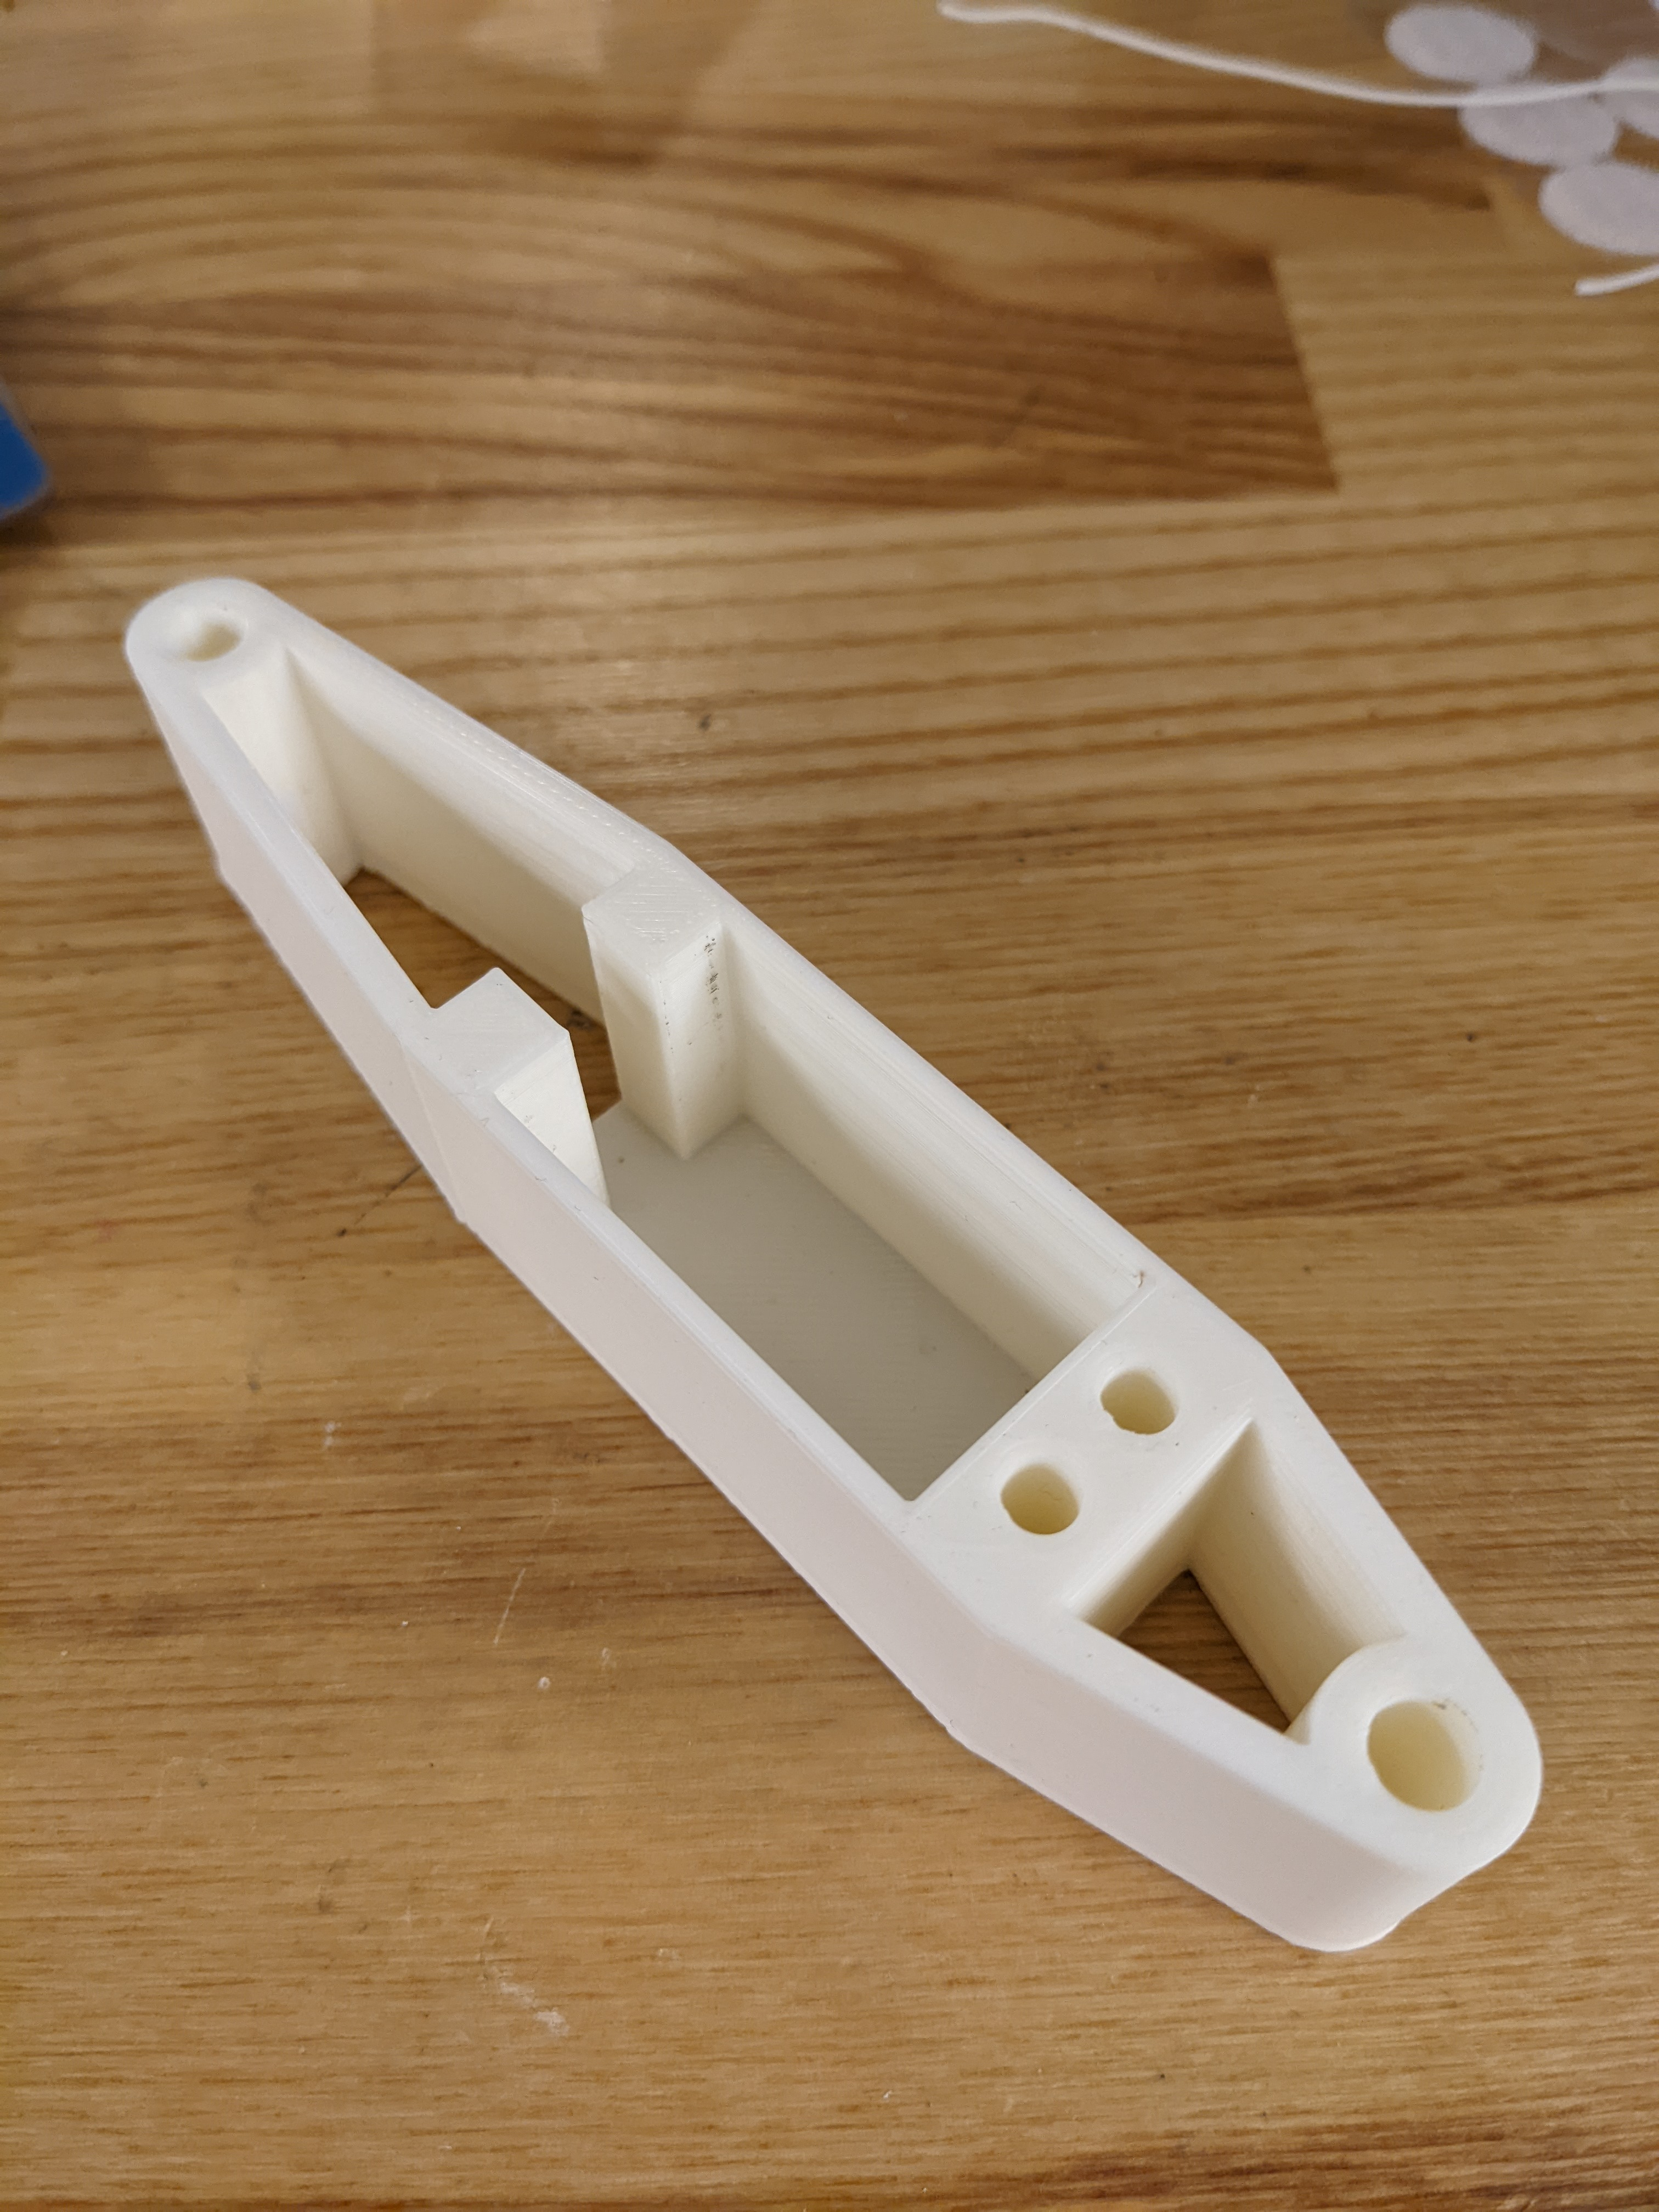
\includegraphics[width=0.75\textwidth]{src/figs/ServoHolder.jpg}
    \caption{Servo Holder}
    \label{fig:SH}
\end{figure}


\paragraph{Deployed Locking Mechanism}
\label{armdeployedlockignmechanism}
Once deployed, the arms need to stay fully deployed to prevent a moving center of thrust, and possibly a blade strike with another component. Several solutions were investigated and the first one selected for testing involved the use of high-strength Neodymium magnets. Magnets were selected due to their fairly cost effective price, reliability (won't fail magnetically), and simplicity of design and installation. Calculations were performed to select magnets that would have the strength to support the moment of the arm and the motor, and magnets that met these specifications were selected. Once ordered, the propulsion arms were modified with a small 11/16" diameter, 1/16" deep circular cutout on the top surface of the arm where it interfaces with the core. This would be the location in which the arm magnet was secured. An accompanying magnet would be secured to the core just above where the arm magnet would fall in the deployed position. The magnets were attached to the arm and core and testing began. The slot for the magnet can be seen in figures \ref{fig:armwspeed}. Initial testing was promising, the magnets were as strong as we expected and could easily hold the arm and motor. Despite this early success, problems arose with the magnets during deployment testing. It was found that if the magnets were not perfectly aligned, when the propulsion arm struck the core magnet, it would bounce off since the magnets did not meet flush. This resulted in fairly serious oscillations of the arms that lasted up to several seconds. After these tests, the magnet idea was scrapped and the team began researching new methods. 

\begin{figure}[H]
    \centering
    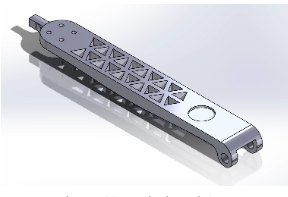
\includegraphics[width=0.75\textwidth]{src/figs/armwithspeed.png}
    \caption{Arm with Magnet Slot}
    \label{fig:armwspeed}
\end{figure}

Two promising ideas were quickly developed and printed for testing. The first idea involved a protrusion from the core that would allow the arm to move into the locked position but not the other way. The second idea involved the use of a spring plunger pin. The pin would be secured to the arm and held in its compressed position while the arm was stowed. Once deployed, the pin would run along the arm bay wall of the core before deploying into a cutout when the arm reached its fully deployed position. Since this mechanism was only concerned with not letting the arm fall, the team was not concerned with the loading it would take since the thrust force would not be sent into it and instead into the core. The pin would be secured to the underside of the arm using a press fit holder that would attach to the arm via two small bolts. After printing new cores that would accommodate these mechanisms, both were tested. It was found that design \#1, the core tabs, was too stiff and too brittle. When deployed, the arm did not pass through the tabs and if pushed through, the tabs would crack. Design \#2, the spring pin, was found to work great and reliably locked the arms in the deployed position (more on testing in the testing section). Design \#2 was selected for further development. The deployed position of the mechanism can be seen in figure \ref{fig:armlocked}.

\begin{figure}[H]
    \centering
    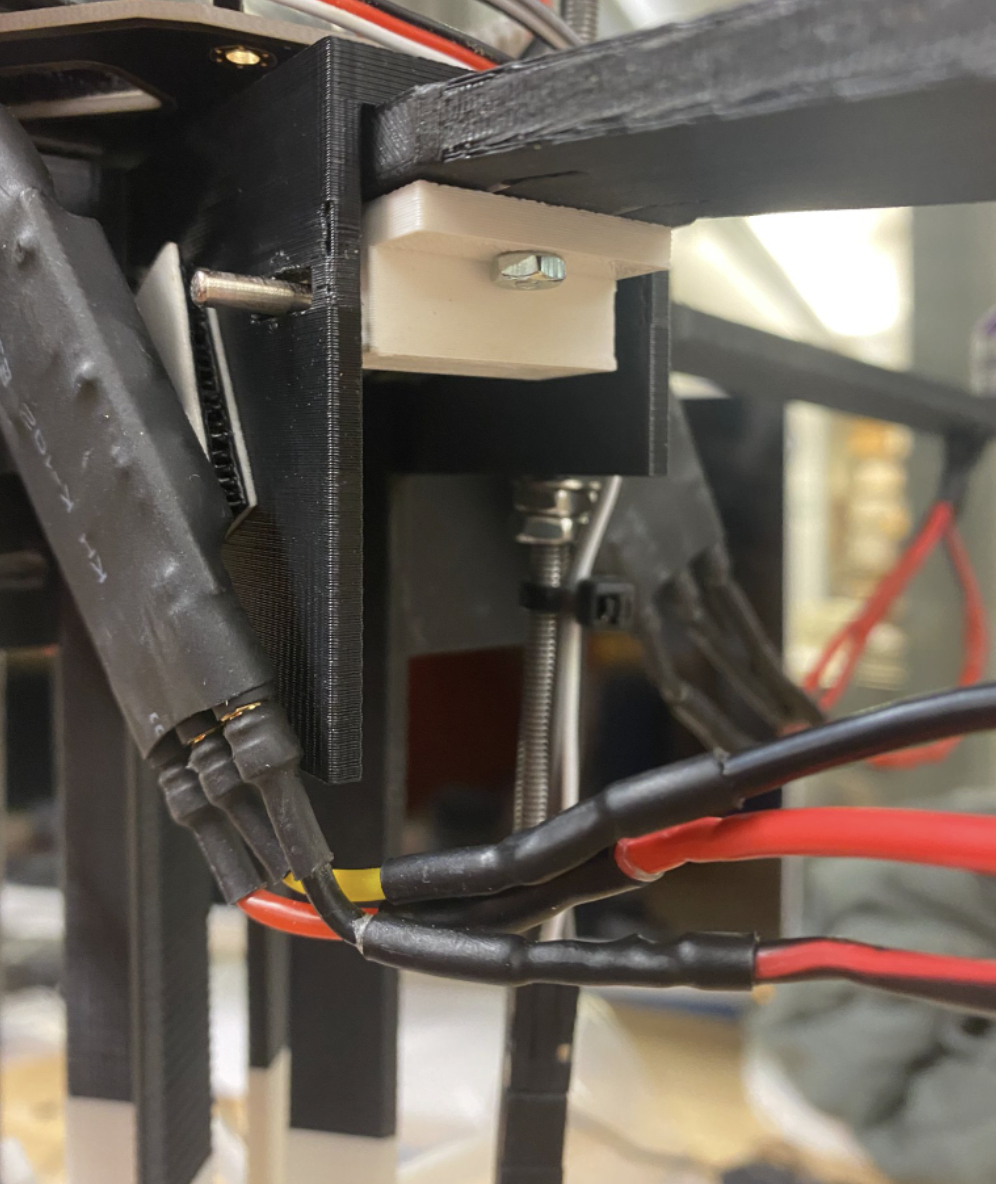
\includegraphics[width=0.75\textwidth]{src/figs/deployedarmimageview3.png}
    \caption{Locked Arm Position}
    \label{fig:armlocked}
\end{figure}



For iterations of this locking mechanism, changes to the initial spring pin design were minimal, and only involved reducing the core cutout size to prevent any vertical motion of the arm and adding countersunk M3 holes to the arm to secure the spring pin holder to it. This design is present in the alpha prototype. 

\subsection{Core}
From the mid-point of Quarter 1, the team decided that simplifying assembly and disassembly would be helpful for maintenance and replacement of internal components. However, it wasn't until Quarter 2 that development of a mechanism to fulfill this requirement began. The initial design was made of 4 propulsion arm bays. These bays were 1.5" wide and consisted of three vertical walls and one top surface. The two side walls were in place to prevent the propeller blades from rotating before deployment. The third vertical wall was located more central than the arms inside the rocket. This wall provided a surface for the other end of the torsion springs to push against to deploy the arms. Finally, the top surface provided a support for the arm so it could not travel beyond its fully deployed position. The design had two holes in each bay to allow a fastener to pass through and secure the arm in its place in the core. Additionally, two supports were added to the exterior faces of two of the walls with a 1/4" through hole to allow the core to mount on 1/4" threaded internal rails (discussed in coming sections) to allow for easy removal.

Since this design, the concept of the core has remained nearly identical with four bays each made of three walls and a top surface. The most drastic design change came with the switch from 90 degree to 120 degree torsion springs for arm deployment. The team wanted the springs to be at their free angle when the arms were fully deployed. To allow for this, the inner walls of the core were slanted 30 degrees towards the center so that when the arm is deployed to its 90 degree deployed positions, the springs are in their 120 degree position. In addition to this change, small tabs were added to the slanted face to prevent the springs from slipping out of place which could prevent proper arm deployment. Additional changes have included narrowing the bays from 1.5" to 1.25", shortening the vertical walls and instead adding 'blockers' that extend below the core to prevent rotation of the blades, and adding the cutouts for the propulsion arm deployed locking mechanism. The alpha prototype is 3D printed using high infill ABS. Each bay provides structures to support the propulsion arm, the deployment method, and the deployed-locking mechanism. Additionally, the extra space on the walls of the bays and top surface are used for mounting the electronic speed controllers as well as the power distribution board.

\paragraph{Avionics Sled}
To support the remaining avionics, a flat plate was printed that could be mounted vertically inside the rocket body on the internal support structures. This component was originally 4.5" wide and 6" tall (figure \ref{OES}. In the mass saving process, this component would be combined with the lower support plate, discussed in the following section. 

\begin{figure}[H]
    \centering
    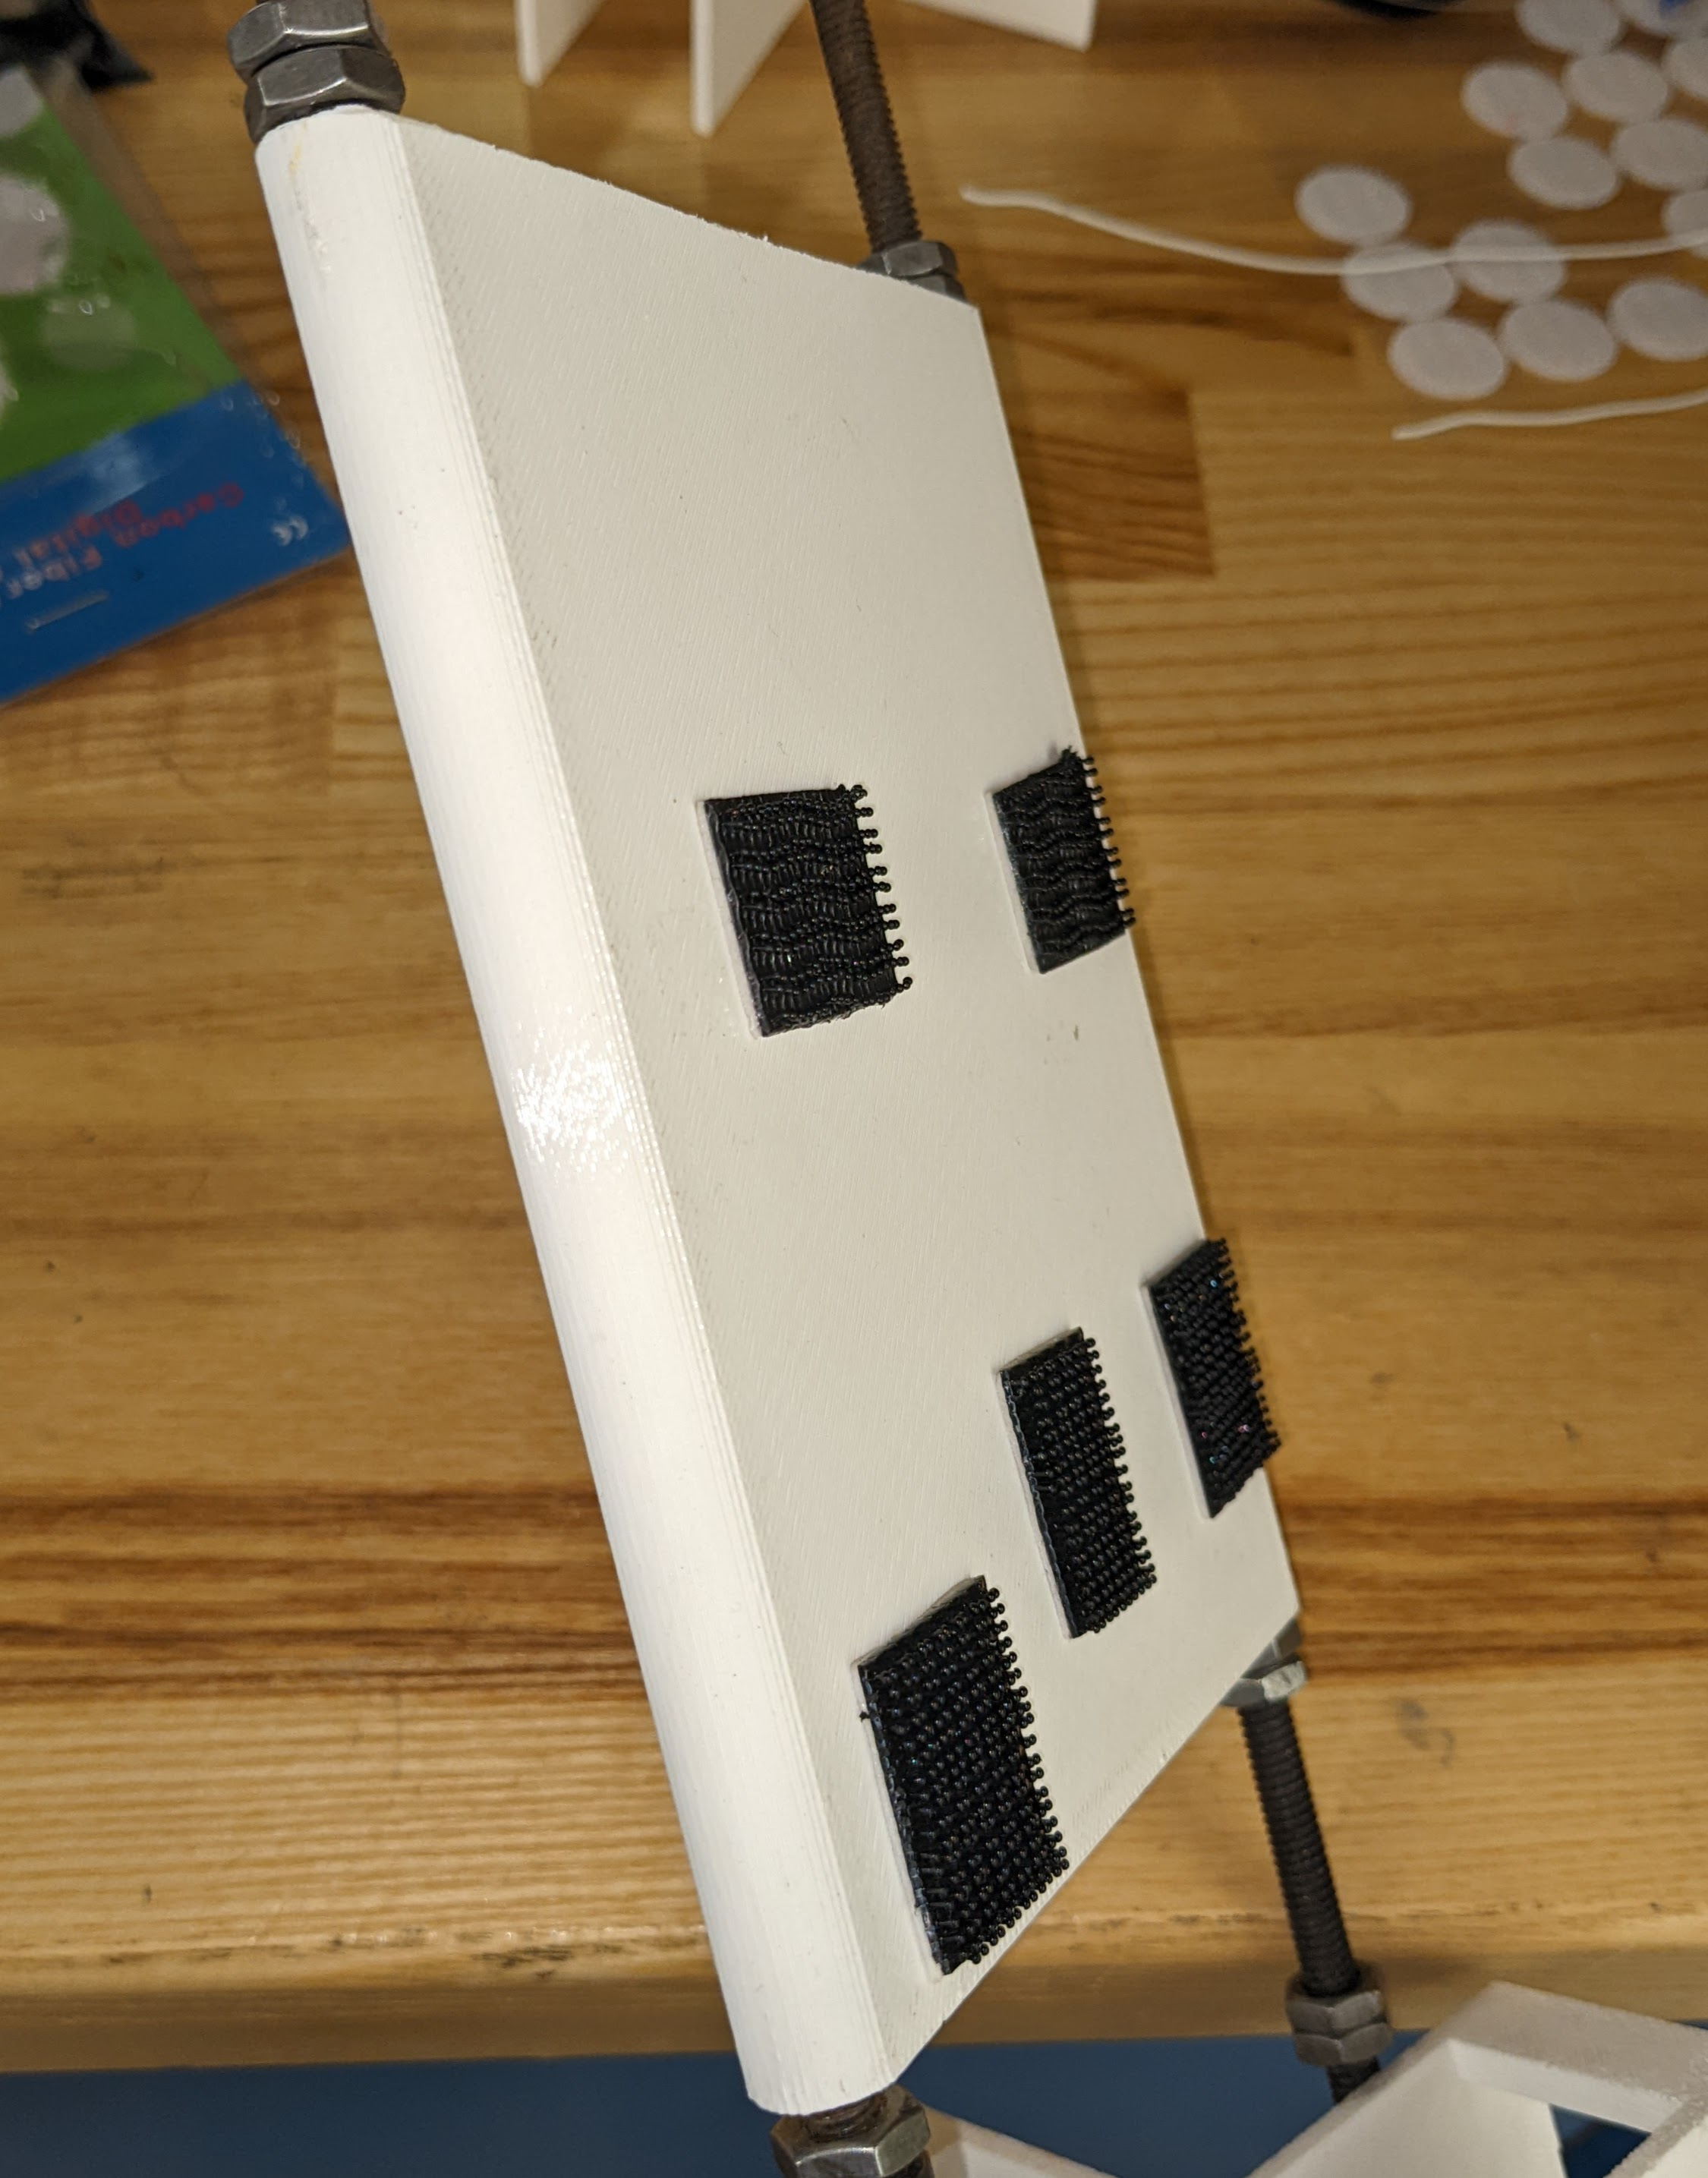
\includegraphics[width=0.5\textwidth]{src/figs/OldElectronicSled.jpg}
    \caption{Original Electronics Sled}
    \label{fig:OES}
\end{figure}


\subsection{Inner Assembly Support Plates}
To facilitate easy removal of internal components, the team designed a system that would combine all internal elements into one module that could be put in or out of the rocket body all at once and then the individual components could be disassembled. This module involved using two support plates and two threaded rods. The two support plates were 6" in diameter to match the inner diameter of the rocket tube. They each had two, 1/4" holes. The threaded rods for mounting the components passed through these holes and were secured on both sides with shouldered nuts. along the outer face of each plate, 8 pilot holes were printed. These holes were expanded and M3 threaded inserts were added to secure the plates to the rocket body. They were secured by passing M3 screws through the body tube and into the plates. Connecting the two plates, were two, 1/4" threaded steel rods. All internal components were slid onto these rods and secured using shouldered nuts. This system remained unchanged until the mass saving process. At the end of Quarter 2, to reduce mass, the threaded 1/4" steel threaded rods were swapped for \#10-32 aluminum threaded rods. This reduced the mass of the rods by approximately 25\%. Additionally, the upper support plate was combined with the avionics sled and the lower support plate was printed to accommodate the leg and arm deployment servo. The alpha prototype is made of two support plates, one that houses the avionics and one that houses the deployment servo. These plates are connected by two \#10-32 rods and secured to the rocket using 16, M3 screws.

\section{Landing Leg System}
The Landing Leg System was the final of the three main systems to enter the design stage. Development of the landing legs began around week 15 of the project. Numerous designs were developed, tested, evaluated and either scrapped or iterated on. The final landing leg assembly is shown in Figure \ref{figs:legassemble}. 

\begin{figure}[H]
\centering
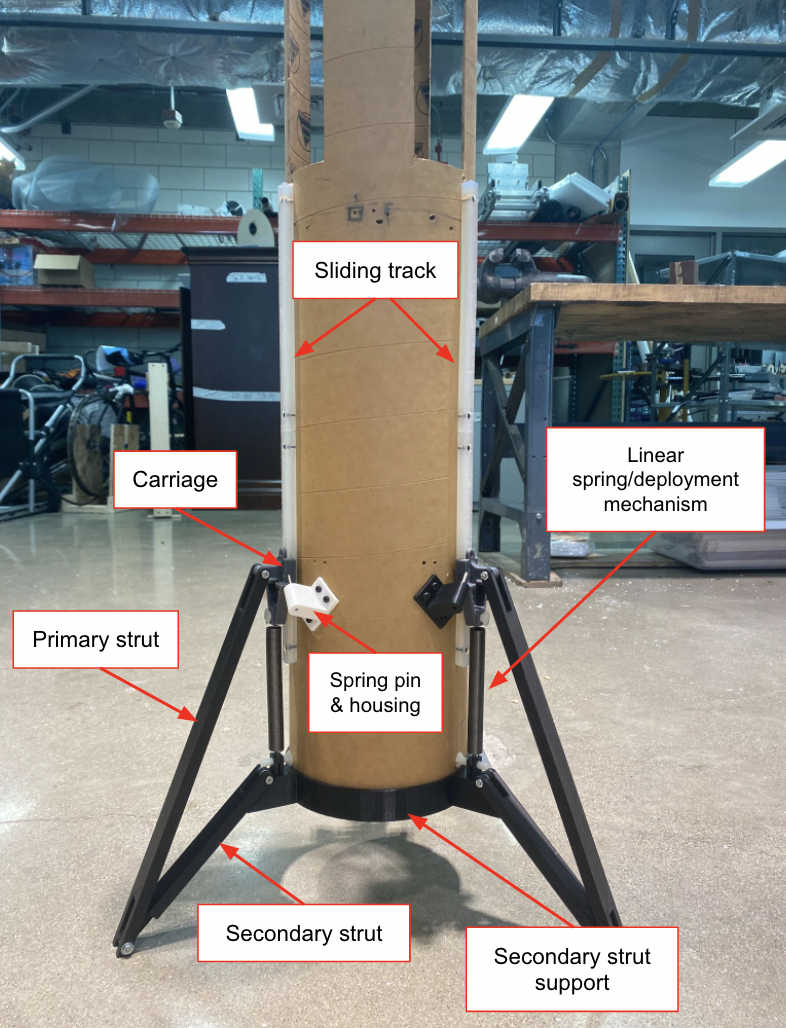
\includegraphics[scale=0.7]{src/figs/overviewlandinglegpiclabeled.png}
\caption{Alpha Prototype of the Landing Legs with Labels}
\label{figs:legassemble}
\end{figure}

The purpose of the landing legs is to support the rocket body upon landing and ensure that the rocket body lands upright in a stable position. The needs that the landing legs must meet are \#3, the ability to stand upright on its own, \#7 reproducible on a college club budget, \#8 structural stability, and \#12 deployability. The team broke down the landing leg design into three separate functions: structural design for load bearing and landing upright, deployment of the legs from an initial stowed position, and two different locking mechanisms to lock the legs in their stowed position and their deployed position. These separate functions were brainstormed and ranked independently. Once solutions that best met the mission's needs were highlighted, they were combined with the other function's solutions and ranked once again. 
The following sections detail this process and what steps were taken to get to the alpha prototype.

\subsection{Structural Leg Design}

The structural leg design investigated different deployment motions and load-bearing structural components that would minimally interfere with the rocket body and other mechanical and electrical components, allow for quick deployment, minimize stress at concentration points, and have minimal complex geometries and manufacturing techniques. A common landing leg design in the aerospace industry includes a primary strut that acts as the main load-bearing element and a secondary strut that provides additional support especially in the axial direction. The other possible design that fit our project includes a single load-bearing strut. The deployment motions possible with these designs include rotation that is tangent to the rocket body, deployment outwards using the bottom of the rocket body as a hinge/rotation point, stowing the legs inside of the rocket body and deploying them from the bottom outwards, and deploying the legs outwards from the upper section of the rocket body (Figure \ref{figs:dm}).

\begin{figure}[H]
\centering
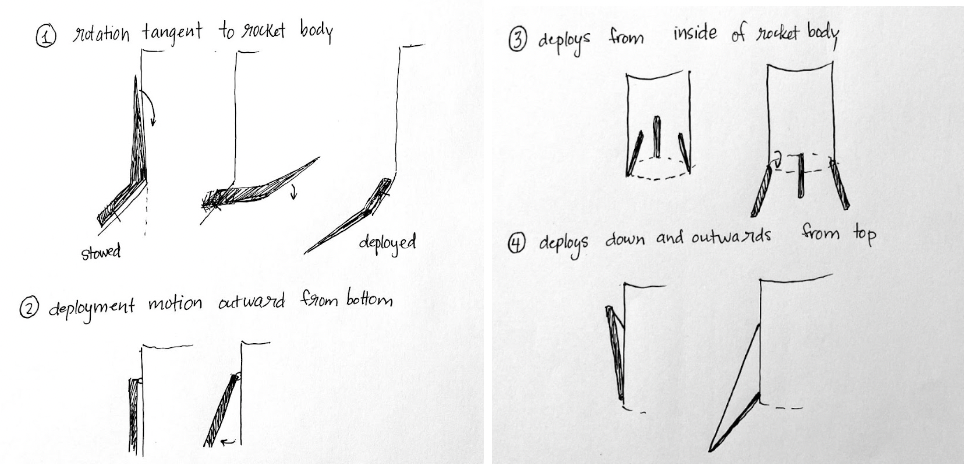
\includegraphics[scale=0.8]{src/figs/deploymentmotions.png}
\caption{Deployment motions}
\label{figs:dm}
\end{figure}

The needs of the landing leg design highlighted above indicates that the primary-secondary strut solution was best fit for the project mission because it is simple, distributes forces on two connection points to the rocket body which reduces shear stress, and reduces bending stress when compared to a single strut while increasing the rocket's stability/footprint. The deployment motions that best meet the landing leg's needs are ideas 2 \& 4. Idea 1 limits the geometry of the strut, sacrifices stability, and would likely interfere with other components when rotating about its axis. Idea 3 causes the legs to be directly in the path of a theoretical thruster, making it unacceptable for the NUSTARS project application. Ideas 2 \& 4 are best suited to the project. The next step in designing the landing legs was to investigate and select potential solutions for the deployment method.

\subsection{Deployment Methods}

The deployment method directly meets the deployable need of the legs outlined above. It is a mechanism that provides a force to initiate the motion of the legs from their stowed position to their final deployed position. The deployment method needs to be lightweight, simple, quickly able to deploy the legs, need minimal support from additional structures, reusable, reliable, and able to apply a sufficient force (or energy) to deploy the leg. The potential solutions and their scores against each need are shown in Figure \ref{figs:dmam}.

\begin{figure}[H]
\centering
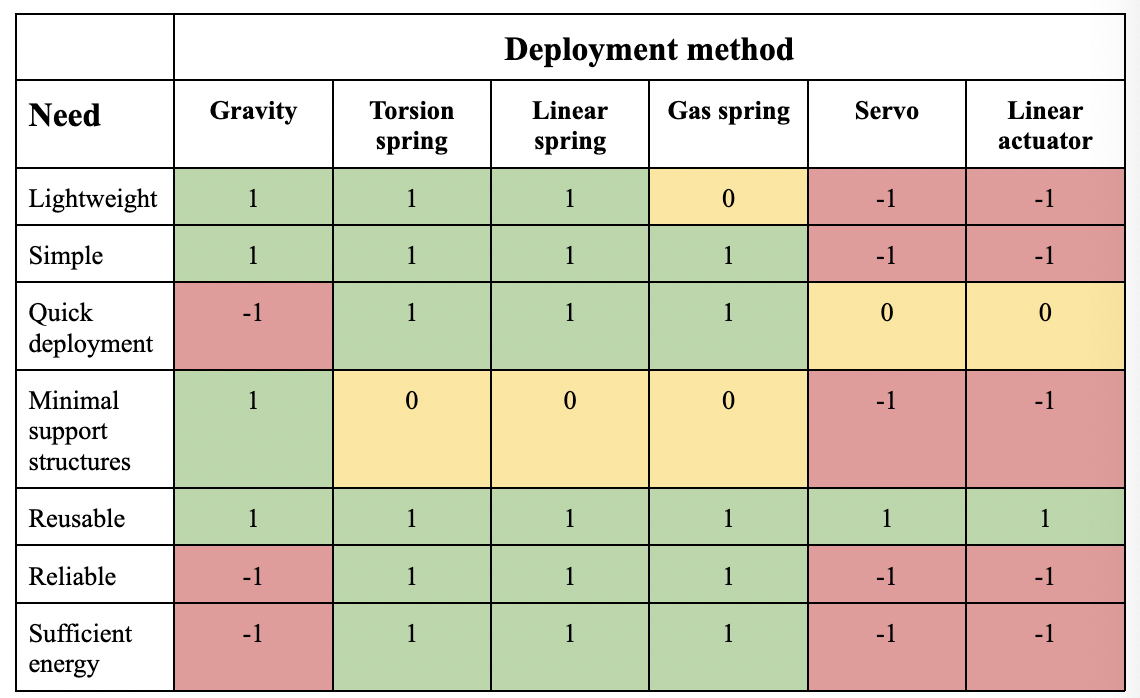
\includegraphics[scale=0.7]{src/figs/deploymentmethodalternativesmatrix.png}
\caption{Deployment Methods Alternatives Matrix}
\label{figs:dmam}
\end{figure}

The two solutions that ranked the highest are to torsion spring and linear spring. Next, the general locking mechanism was investigated. 

\subsection{Locking Mechanism}

The locking mechanism refers to the component of the landing legs that constrain the motion of the leg before and after deployment. Similar to the deployment mechanism, the needs are lightweight, simple, minimizes stress at connection points, locks the legs quickly, minimally supported by additional structures, reusable and reliable. 

\begin{figure}[H]
\centering
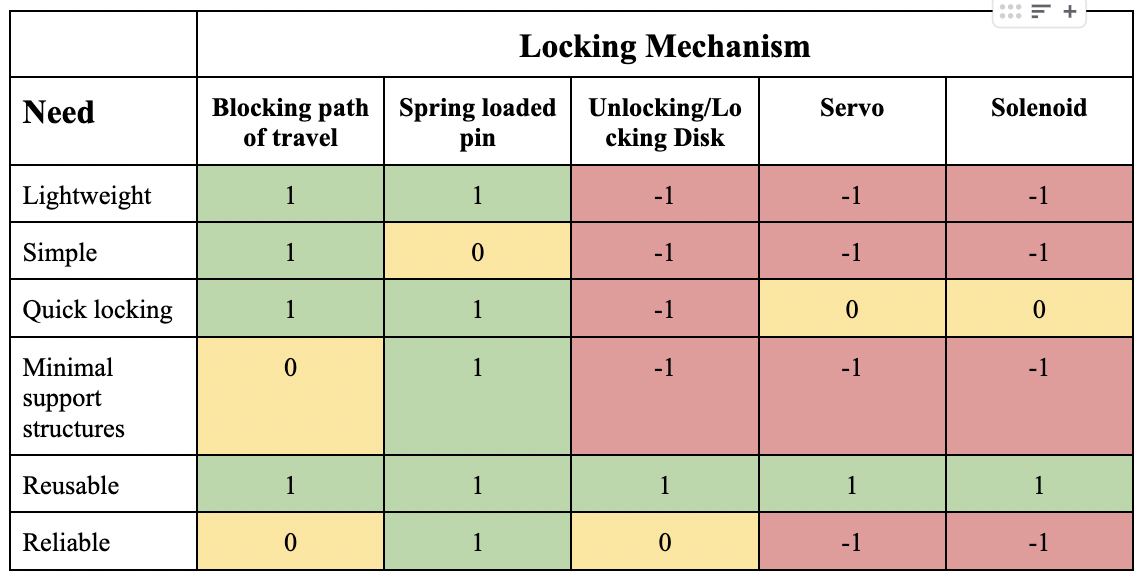
\includegraphics[scale=0.8]{src/figs/lockingmechanismalternativesmatrix.png}
\caption{Locking Methods Alternatives Matrix}
\label{figs:lmam}
\end{figure}

Figure \ref{figs:lmam} shows the best solutions are a structure that blocks the path of travel of the landing leg and the use of a spring loaded pin. 

The next step was combining these functions and top potential solutions into a single landing leg design and ranking them. 

\subsection{Landing Leg Configurations \& Mockups}

Different combinations of solutions were combined into landing leg configurations and ranked according to how they met the following needs: lightweight, load resistance/the ability to withstand load, aerodynamic efficiency (minimal protrusions from the rocket body), simple/easy to manufacture, and thrust interference. The complete set of configurations is shown in Figure \ref{figs:llc} with detailed views of a top contender shown in Figure \ref{figs:llc1}.

\begin{figure}[H]
\centering
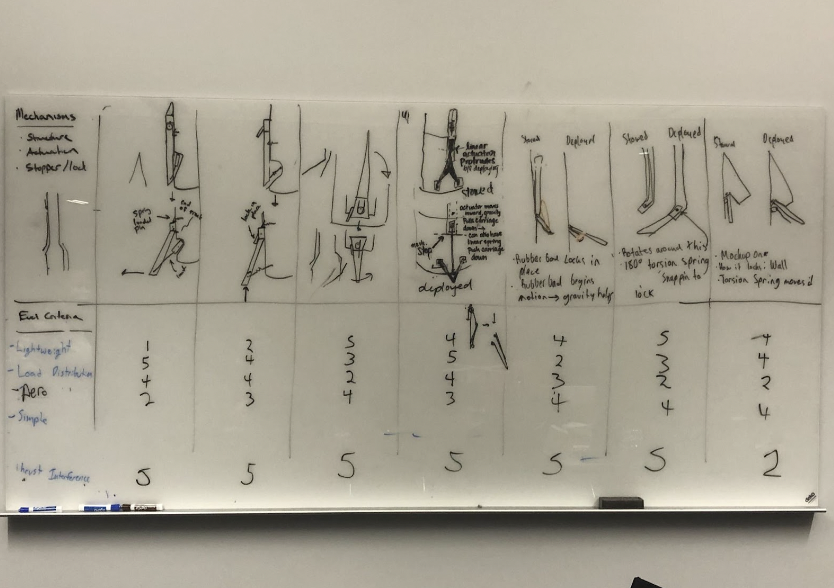
\includegraphics[scale=0.8]{src/figs/configs.png}
\caption{Landing Leg Configurations}
\label{figs:llc}
\end{figure}

\begin{figure}[H]
\centering
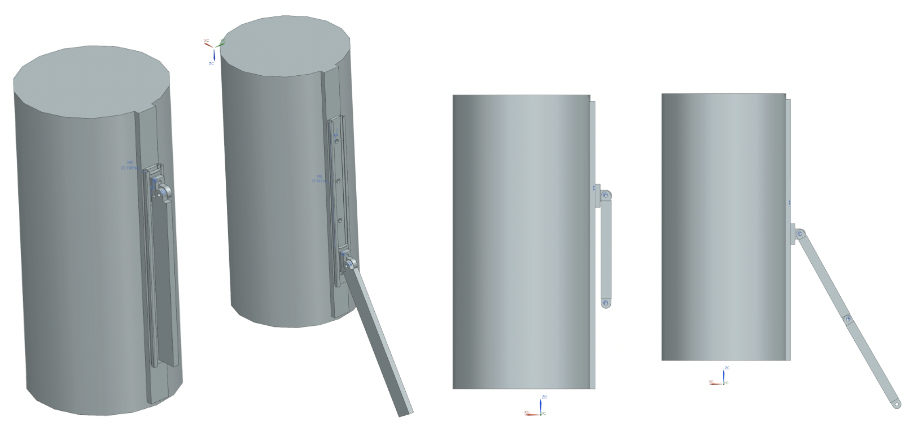
\includegraphics[scale=0.8]{src/figs/landinglegconfig1.png}
\caption{Configuration 4}
\label{figs:llc1}
\end{figure}

Figure \ref{figs:llc} displays the the top ranking solution as Idea 4. In brief, it utilizes a sliding track and carriage system to move the primary strut down and away from the rocket body. Concept 4 from the whiteboard discussion was chosen to move forward based on its ability to meet the project's needs, its deployment motion, and its ability to be integrated with different locking mechanisms and deployment methods. It had the most promise because each of its components were lightweight (or could be designed to be lightweight), it used gravity to aid in deployment, the parts could be connected with simple pin supports, and a deployment method could be placed either directly underneath the arm or directly above the arm, e.g. a linear spring. The modularity of concept 4 placed constraints on the deployment motion, but allowed the team to create alternative matrices for the other components. A challenge with separating the design of the landing legs into deployment motion, deployment method, and locking mechanism is that these components depend on each other. By selecting one of these components (the deployment motion), the deployment method and locking mechanism could be evaluated within the scope of concept 4’s broad design and layout. The iterative design process continued and new (and old) deployment mechanisms and locking mechanisms were ranked within concept 4's scope [Figures \ref{figs:c4dmam}, \ref{figs:c4lmam}, \ref{figs:c4lmstowed}]. 

\begin{figure}[H]
\centering
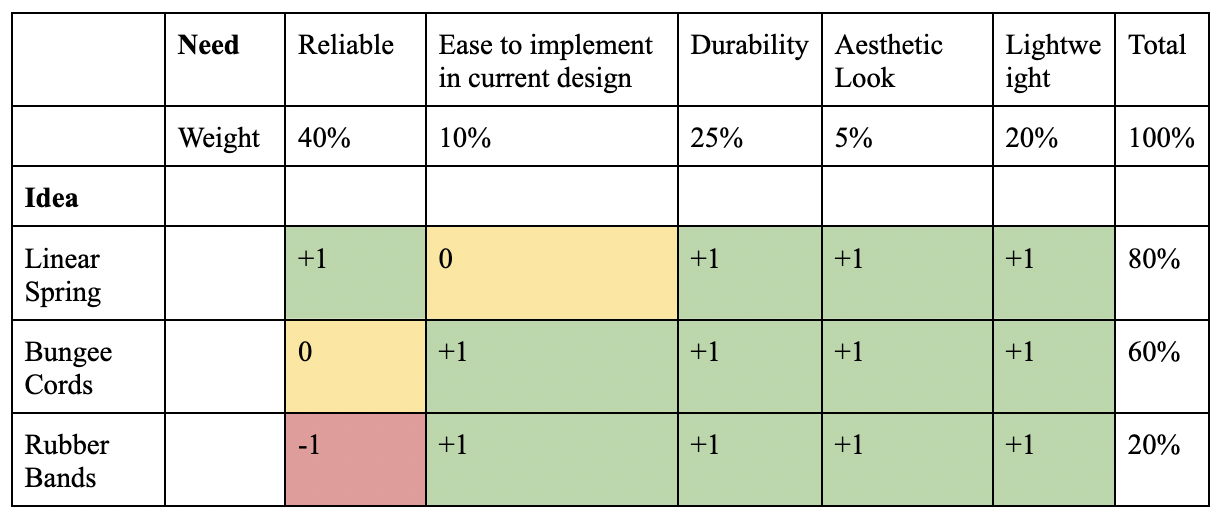
\includegraphics[scale=0.7]{src/figs/Concept4dmam.png}
\caption{Configuration 4 Deployment Method Alternatives Matrix}
\label{figs:c4dmam}
\end{figure}

\begin{figure}[H]
\centering
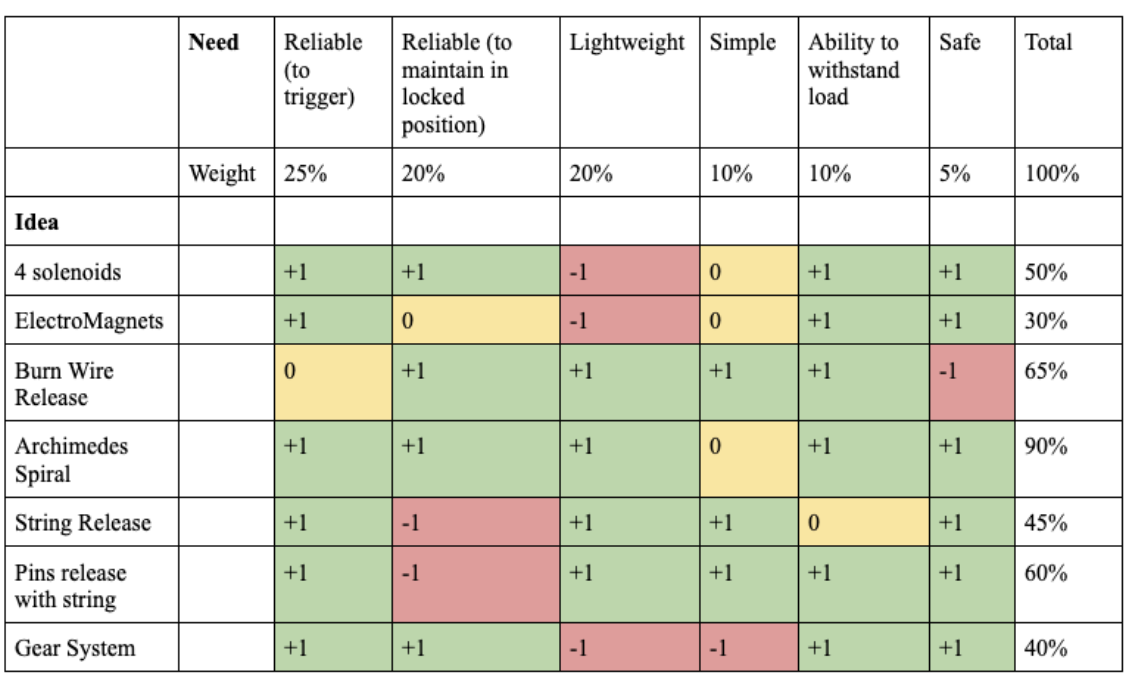
\includegraphics[scale=0.8]{src/figs/concept4lmam.png}
\caption{Configuration 4 Locking Method in Stowed Position Alternatives Matrix}
\label{figs:c4lmam}
\end{figure}

\begin{figure}[H]
\centering
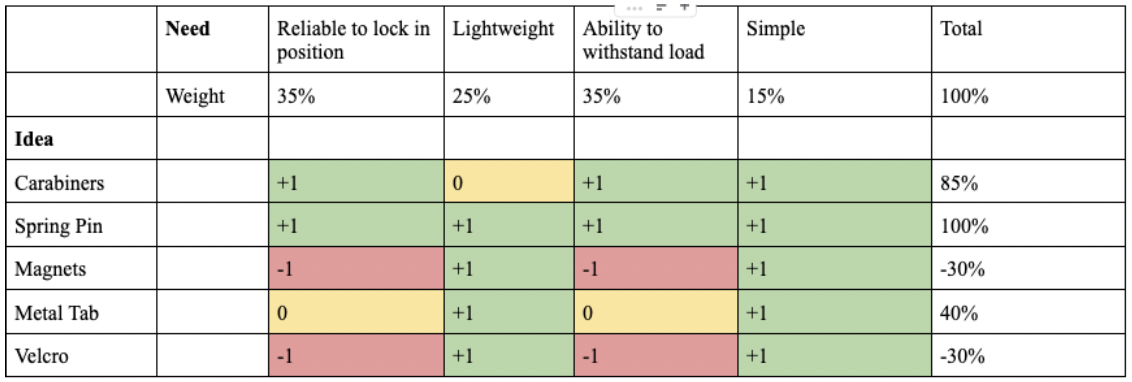
\includegraphics[scale=0.8]{src/figs/concept4lmstowed.png}
\caption{Configuration 4 Locking Method in Deployed Position Alternatives Matrix}
\label{figs:c4lmstowed}
\end{figure}

\noindent The deployment method selected was the linear spring because, although it tied with bungee cords, it was more robust and fitting for the alpha prototype. It was also more reliable and accessible. The locking method chosen for stowing the landing legs was a combination of the Archimedes spiral and string release. The locking method chosen for post-deployed landing legs were spring pins. 


\subsection{Struts}
\paragraph{Introduction of Carriage and Track, Secondary Strut Support}

Once the team had decided on the style and motion of the landing legs struts, we knew that the primary strut would have to be able to slide up and down along the length of the rocket body. With this in mind, the team decided that the primary strut would be hinged on a carriage that was able to move in up and down along a track. To prototype this motion, the team quickly designed a primary strut and secondary strut that we estimated would be close to the actual size of the landing leg struts. The team also purchased a track and sleeve-bearing carriage from McMaster-Carr. Once all the components had arrived, this initial prototype was assembled [Figures \ref{figs:llp1}, \ref{figs:llp2}]. 

\begin{figure}[H]
\centering
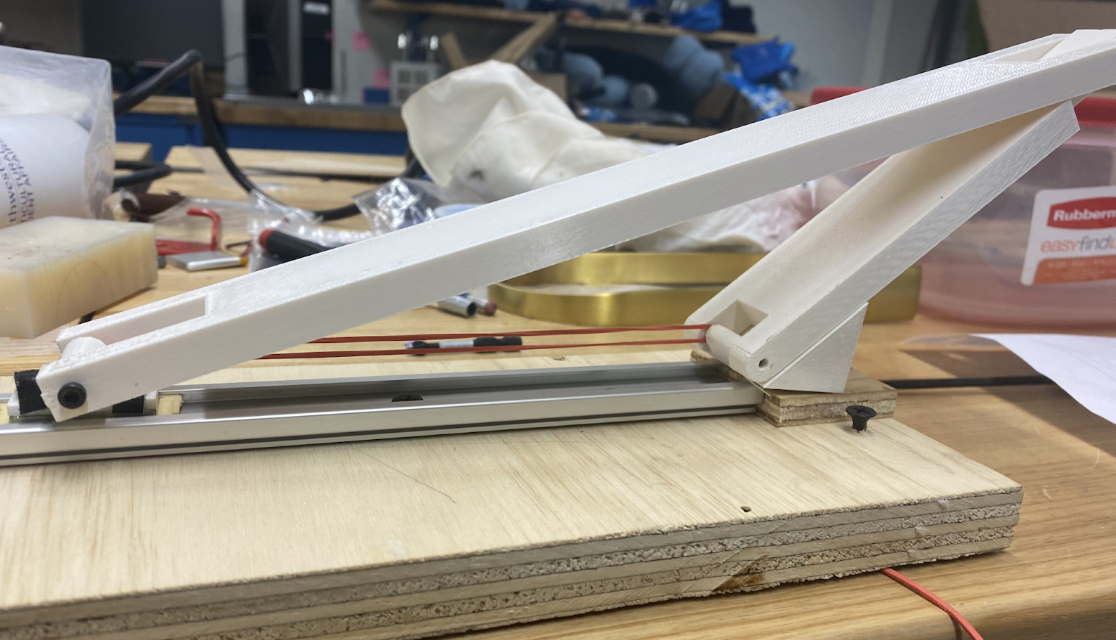
\includegraphics[scale=0.8]{src/figs/landinglegprototype1.png}
\caption{Landing Leg Prototype}
\label{figs:llp1}
\end{figure}

\begin{figure}[H]
\centering
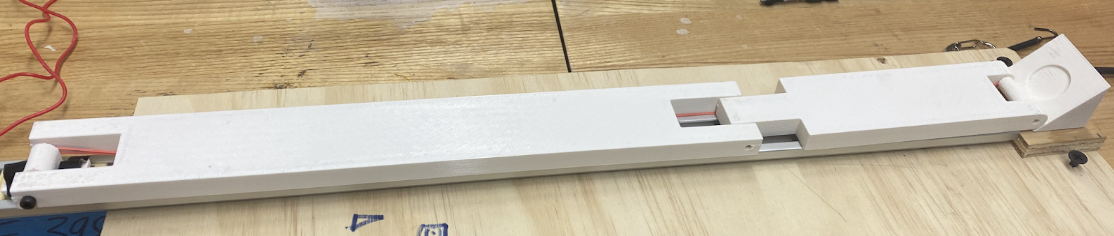
\includegraphics[scale=0.8]{src/figs/landinglegprototype1secondview.png}
\caption{Landing Leg Prototype}
\label{figs:llp2}
\end{figure}

The team tested the prototype and were satisfied with the motion. Using this prototype as a visual aid, the team began looking at deployment methods.

\subsection{Deployment Method}
Since the team had decided on a track and carriage system for allowing movement of the primary strut, it was decided that the most reliable and simple form of deployment would be through the use of either a linear spring or a rubber band to pull the carriage from its stowed position to its deployed position. The rubber band concept was tested using the existing prototype and while it did work, it was found that the rubber bands wore easily and had the tendency to snap unexpectedly. If this were to happen during flight, the leg would likely not fully deploy. With this in mind, the team decided to further investigate linear springs. The driving factor behind selection of the linear spring was the size constraints imposed by the landing legs. Since the linear spring would be positioned between the primary strut and secondary strut, it would have to be no longer than 6 inches in its fully compressed position otherwise it would interfere with the carriage motion. Additionally, it had to be able to stretch to over 12" without deforming when the leg is stowed. With these requirements in mind, the team set out finding the right spring. From McMaster-Carr, several springs meeting this requirement were purchased, all with varying spring constants. To minimize impact loading the leg components, the springs with lower spring constants were selected for testing. Several of these springs were tested and one was selected with a spring constant of 0.4 lbs/in. This spring was the lightest purchased and still provided enough force to pull the leg quickly into its deployed position. The spring is just over 4" fully compressed and can expand to over 13". It has a 0.5" outer diameter and two hooks on the ends for securing it. In the legs fully deployed position, the spring is still in minor tension. This serves to constantly be pulling down on the spring as well as providing minor shock absorption upon landing.

\paragraph{Secondary Strut Support}
To stop the deployment of the landing leg struts at their proper deployed angle, a support was made that constrains the motion of the secondary strut (Figure \ref{original-secondary-strut-support}).This support was designed to stop the secondary strut at 135 degrees of deployment. It was triangular shaped and had a rounded back to match the outer diameter of the rocket body. Additionally, a mount was made so that the secondary strut could be directly mounted to this component through the use of a shoulder bolt. Just above the secondary strut mount, another mount was added consisting of two flat plates that with a small gap between them. Through these plates, a 1/4" hole was added. One end of the deployment spring sits between these two plates and a 1/4" fastener passes through the hole to secure the spring in place. This support mounted to the lower extreme of the rocket body using two M3 bolts that passed through it, the rocket body, and an flat mount plate on the inside of the rocket.

\begin{figure}
    \centering
    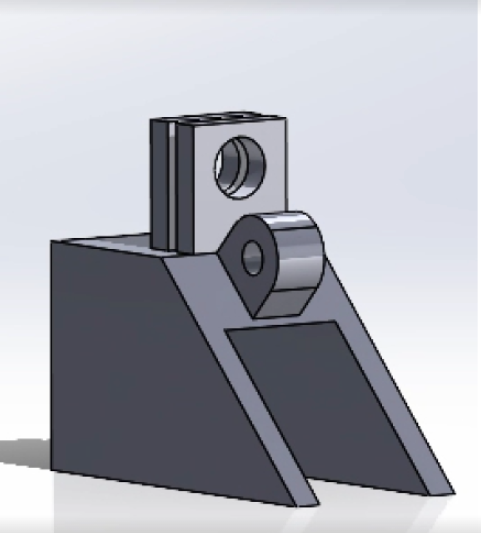
\includegraphics[width=0.6\textwidth]{src/figs/cad-and-dwgs/original-secondary-strut-support.png}
    \caption{First iteration secondary strut support}
    \label{original-secondary-strut-support}
\end{figure}

During testing, the strut support performed well on the first two trials. However, on the third test, the impact force of the secondary strut with the support caused the secondary strut support to collapse the portion of the body tube it was mounted on. It was determined that the cause of this failure was the impact force between the secondary strut and the support. The force of impact could not be easily adjusted since the springs in use were the lowest spring constant available to the team without ordering custom springs. To fix the problem, the team combined all three strut supports into one part with a continuous ring connecting them (Figure \ref{cad:secondary-strut-support} in CAD section). This distributed the load of impact around a greater portion of the body tube to prevent a high stress concentration in one area. 

\paragraph{Pre-Deployment Locking Mechanism}
\label{legpredeploymentlock}
Similarly to the propulsion arms, due to their deployment method, the landing legs naturally want to be in their fully deployed position. In order to stop them from deploying prior to the landing sequence, a pre-deployment locking mechanism was developed. The team wanted to save mass in this process by deploying all 3 legs with a single mechanism, similar to the arms. From this goal, two promising concepts were developed. Both concepts again involved the use a centrally located servo. Both concepts involved constraining the motion of the carriage since only one direction of travel would have to be constrained. Both concepts utilized some form of a pin that was inserted into the back of the leg carriage. When deployment was necessary, the pin was removed from the back of the carriage, allowing it to be pulled into its deployed position. 

The first concept was based off of the motion of a piston in an engine in which two arms were connected at a hinge point and one of the arms was connected to a servo. The servo would rotate and the two arms would be constrained in such a way that the servos rotation would be converted to a 1D linear motion (figure\ref{fig:ALM}). The second concept followed similar suit except instead of having two arms, it relied on a single pin that would be pulled from the back of the carriage via a string or other flexible material. This string would be attached to a centrally located mount that was spun by the servo. The concepts were discussed and for its simplicity, the second concept was selected to be prototyped. 

\begin{figure}[H]
    \centering
    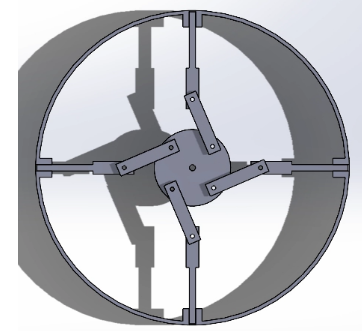
\includegraphics[width=0.5\textwidth]{src/figs/DavidPin.png}
    \caption{Alternative Locking Mechanism}
    \label{fig:ALM}
\end{figure}

A 'spool' was created in SolidWorks that mounted to a servo in the same fashion the propulsion arm locking disk did. The spool had three mounts, one for each legs string. At the end of the string, pins were to be attached that would pass through the rocket body and into the carriage (Figure \ref{fig:OldSpool}). This iteration remained the what was believed to be the final version until the mass saving process began. In this process, the arm deployment and leg deployment mechanisms were combined. With this combination, a small extrusion was made to the top of the spool and pilot holes were added for threaded inserts. The propulsion arm pre-deployment locking disk would slide over this extrusion and be secured using M2 screws in the threaded inserts. This version is present on the alpha prototype and is 3D printed using ABS (figure\ref{fig:curSpool}). 

\begin{figure}[H]
    \centering
    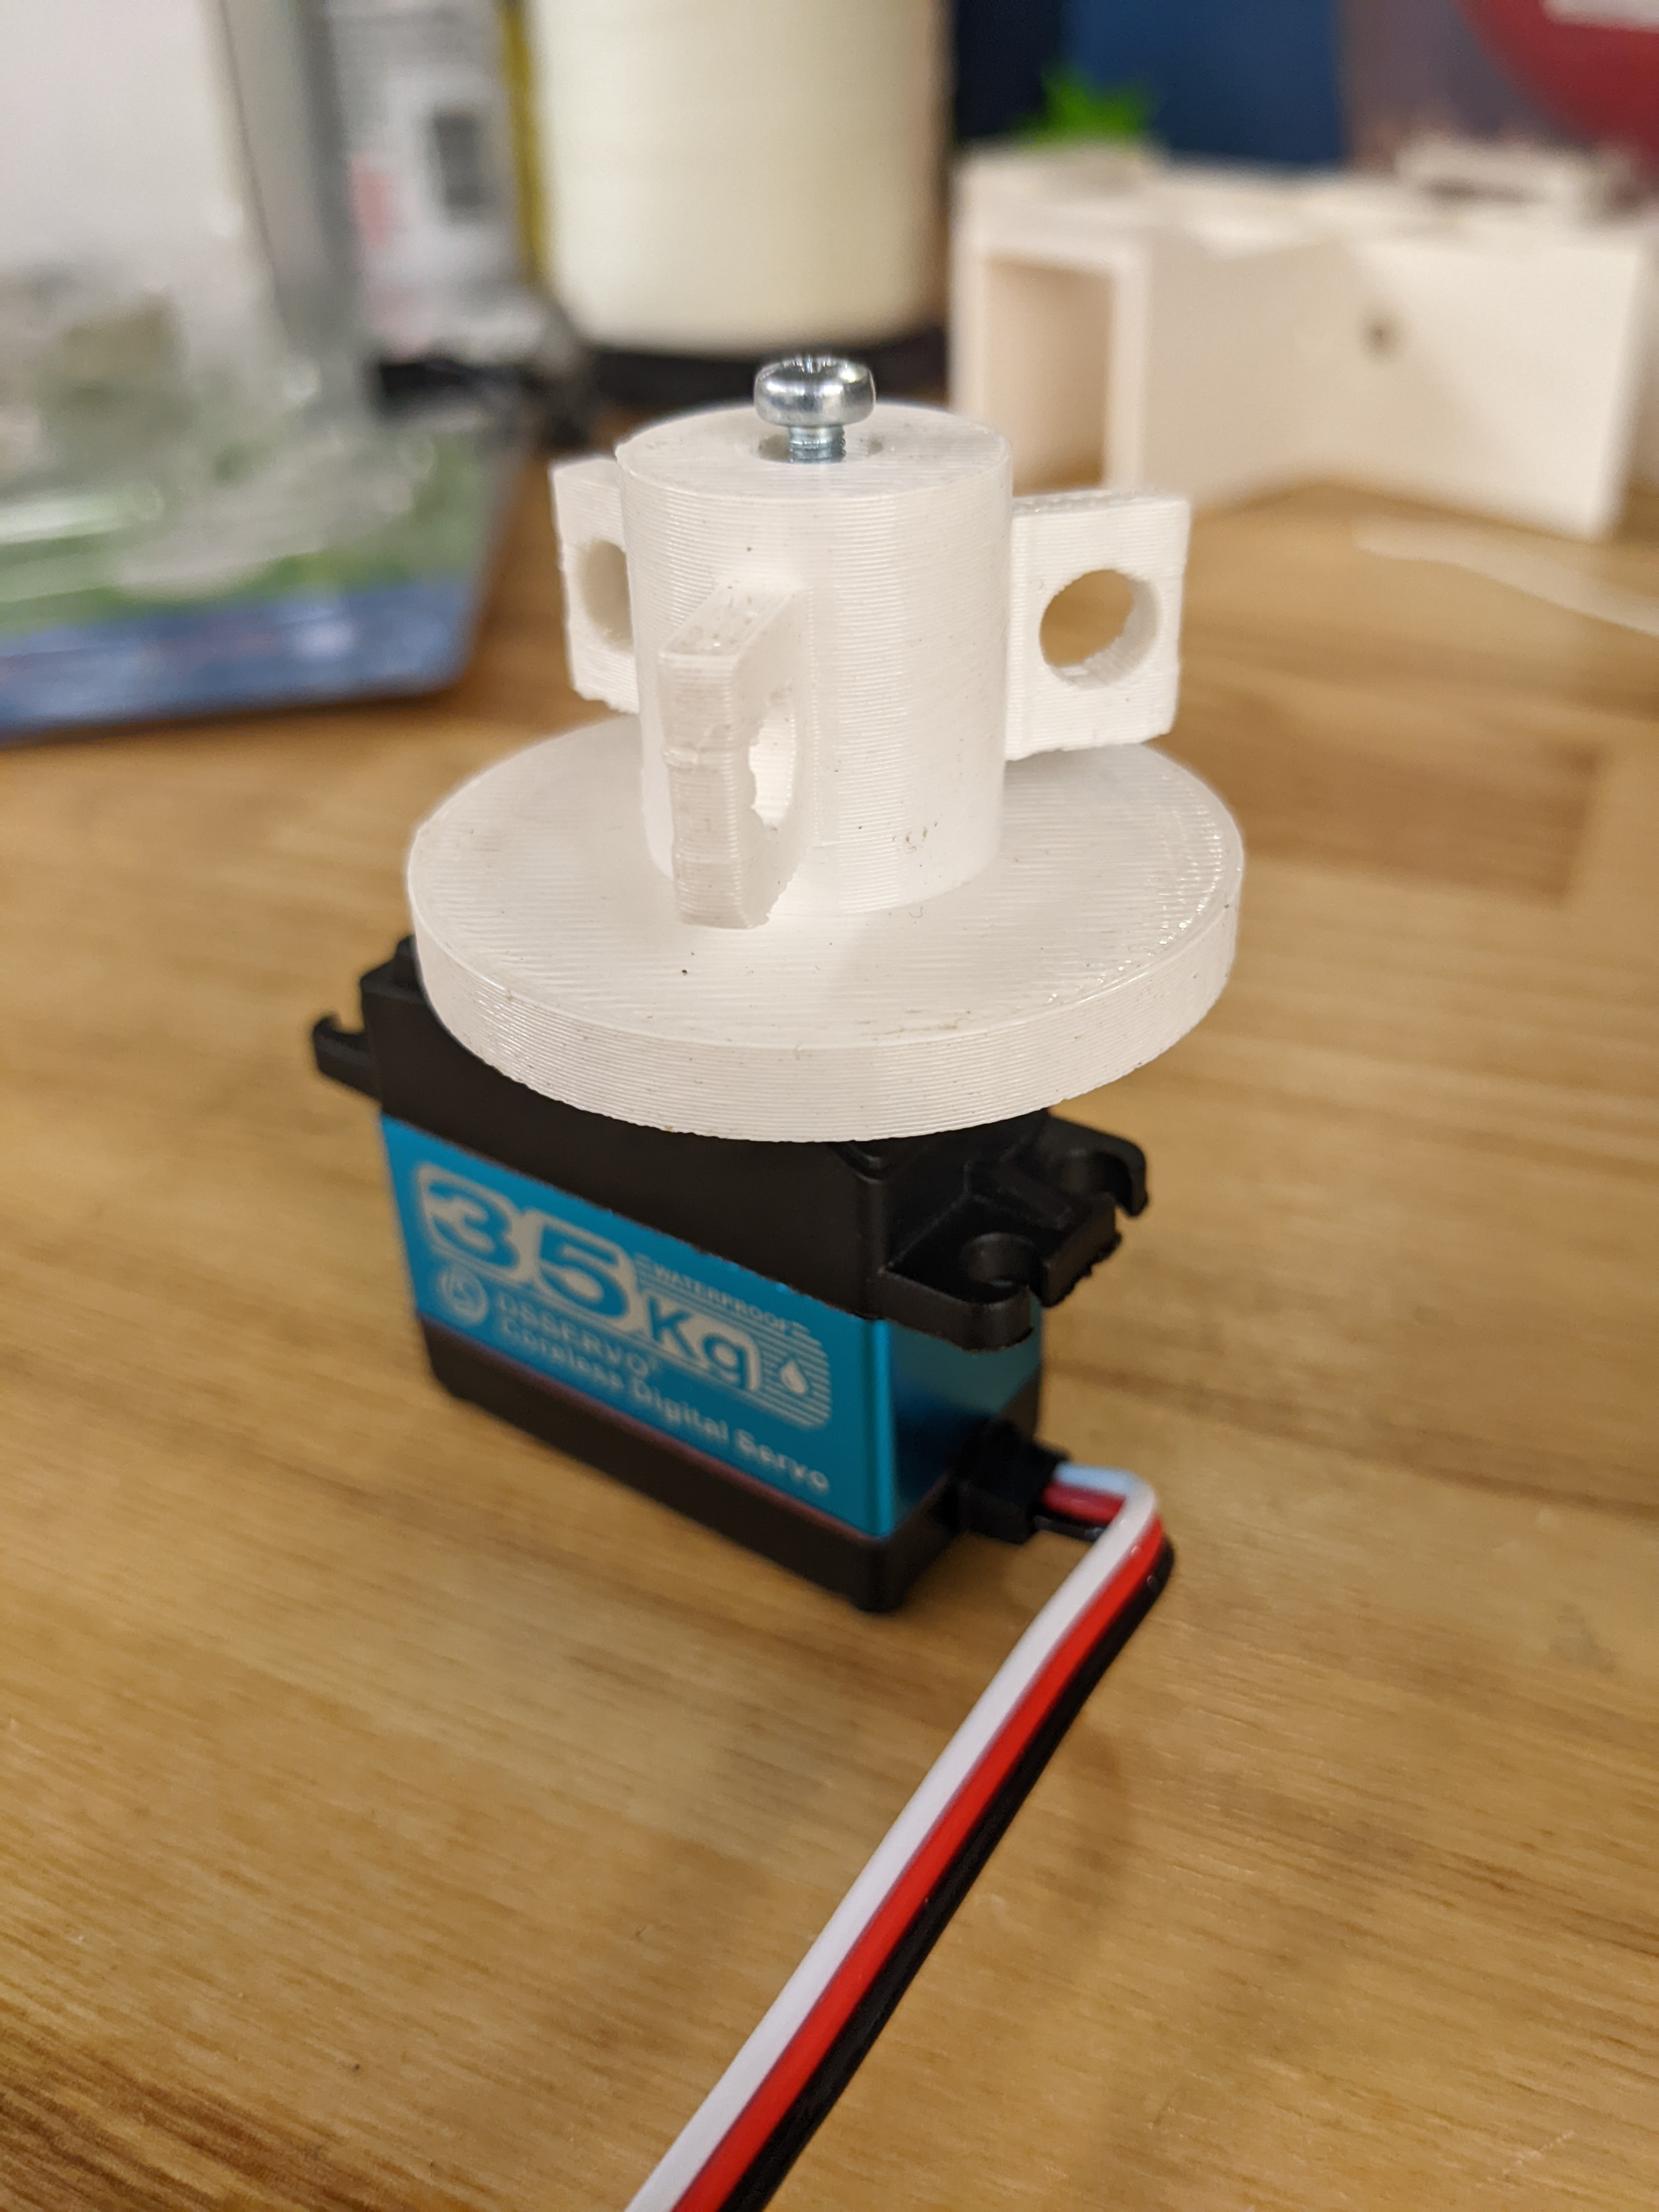
\includegraphics[width=0.5\textwidth]{src/figs/OldSpool.jpg}
    \caption{Old Version of Spool}
    \label{fig:OldSpool}
\end{figure}

\begin{figure}[H]
    \centering
    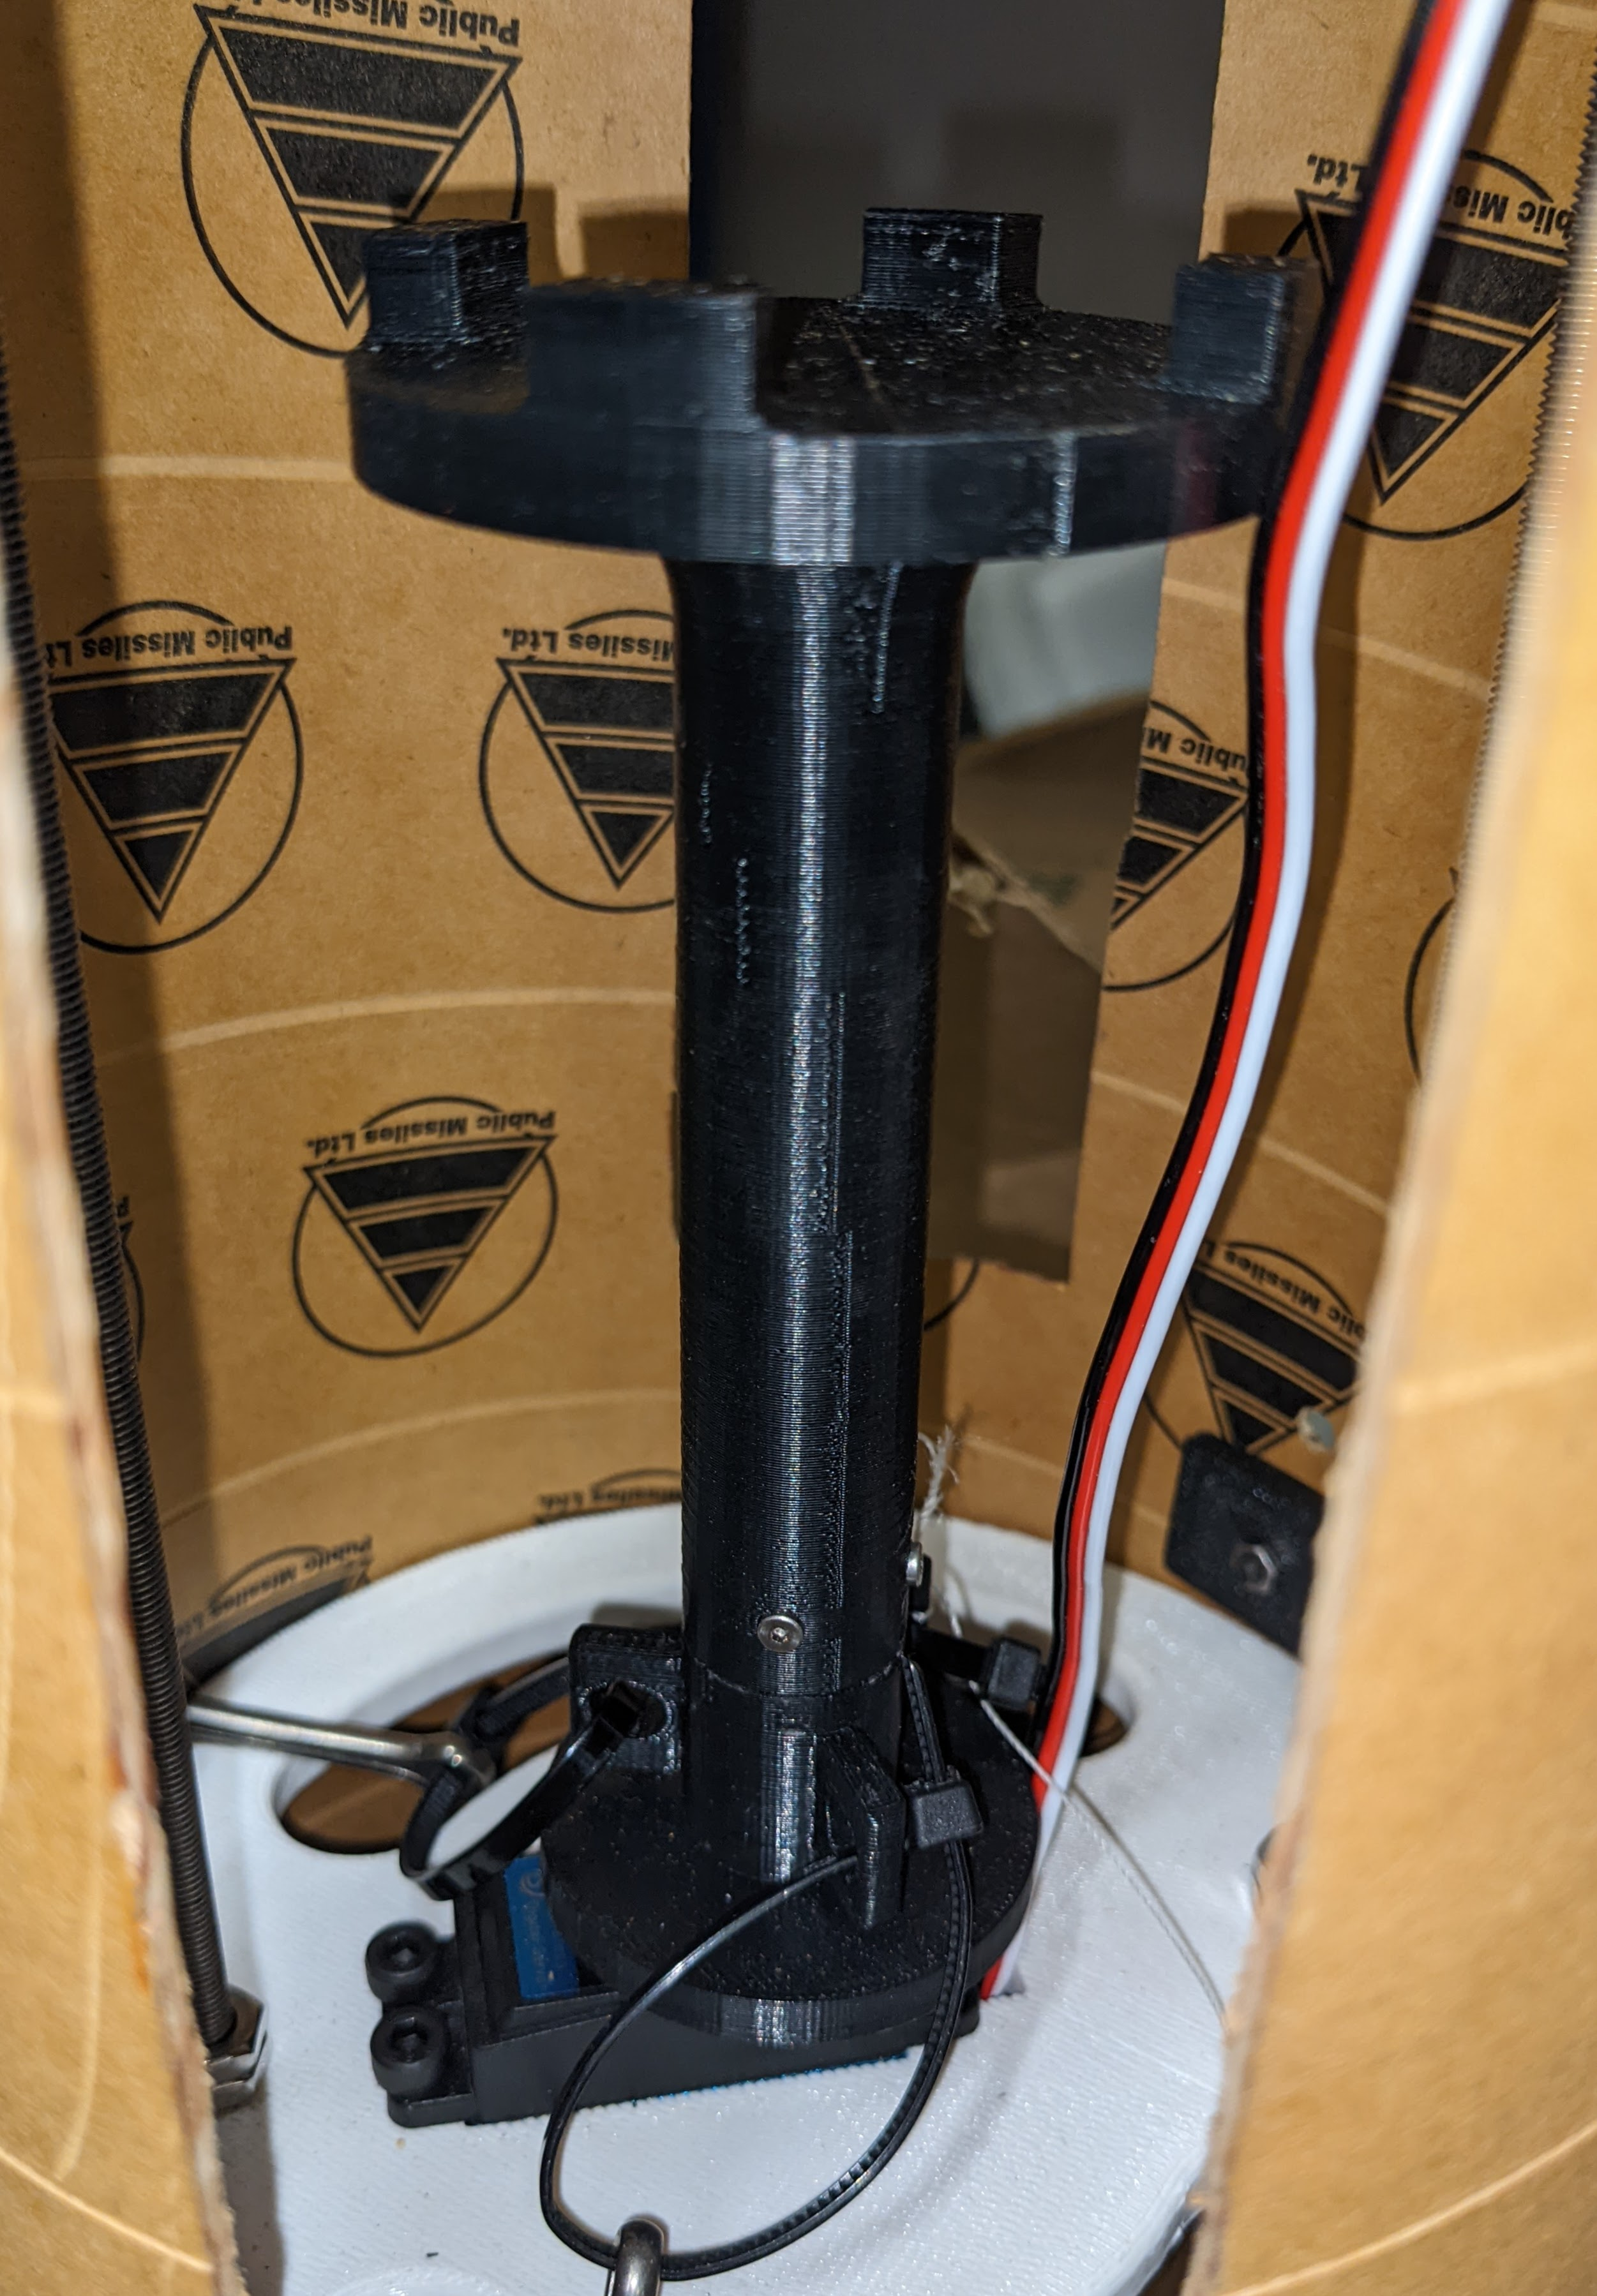
\includegraphics[width=0.5\textwidth]{src/figs/NewSpool.jpg}
    \caption{Current Spool Located into Rocket Body}
    \label{fig:curSpool}
\end{figure}

\paragraph{Deployed Locking Mechanism}
\label{legdeployedlockingmechanism}
Once deployed, the leg needs to be able to stay in its fully deployed position with the weight of the rocket on it as well as with the force of impact at touch down. Several options were looked at and all involved some form a "spring-loaded" mechanism. The two leading contenders were the use of a spring loaded pin, and the use of an elastically deformed piece of metal. In both cases, the carriage would slide by the locking mechanism, deforming it slightly. Once passed, the locking mechanism would return to its original position, blocking the carriage from traveling back up the track. The bent metal idea was quickly eliminated because the team feared that finding exactly the right metal that would bet strong enough to withstand the return of the carriage but also weak enough where it could easily be deformed for the carriage to deploy would be too time consuming of a process and may not even yield any actual results.

The spring pin locking method took two possible forms. One involved the spring pin being mounted under the track and the carriage would hold it compressed. Upon full deployment of the legs, the pin would expand into a cutout in the carriage locking it in place. This idea was promising but it would required a fairly large custom carriage that would hold the pin down throughout its path of travel. The second pin idea involved two pins mounted on both sides of the track and carriage assembly just above the carriage's fully deployed position . The pins would stay in their expanded position until the carriage reached them. At this point, the carriage would impact the pins, compressing them and allowing the carriage to slide past. Once the carriage was fully deployed, the pins would expand, preventing the carriage from returning to any position above them. 

The second concept involving two pins per leg was selected for a number of reasons including better support since the load is distributed on two pins instead of one as well as requiring a much smaller carriage. This concept uses two spring pins in press fit housings. The housing mount to the outside of the rocket body and are shaped so that the surface in contact with the rocket matches the diameter of the tube.

Initially, the spring pins were mounted so that they were perpendicular to the track. However, in testing it was found that this orientation caused a serious problem. When struck by the carriage, the pin was pushed slightly down which prevented it from compressing. This resulted in either the legs not deploying, or a ballistic failure of the carriage. To fix this problem, the pins were mounted facing slightly upwards so that when the carriage struck them, it was more in line with their intended direction of travel. 

The overall design of the pin locking mechanism with them angle upward is shown in figure \ref{fig:lockpins}.

\begin{figure}[H]
    \centering
    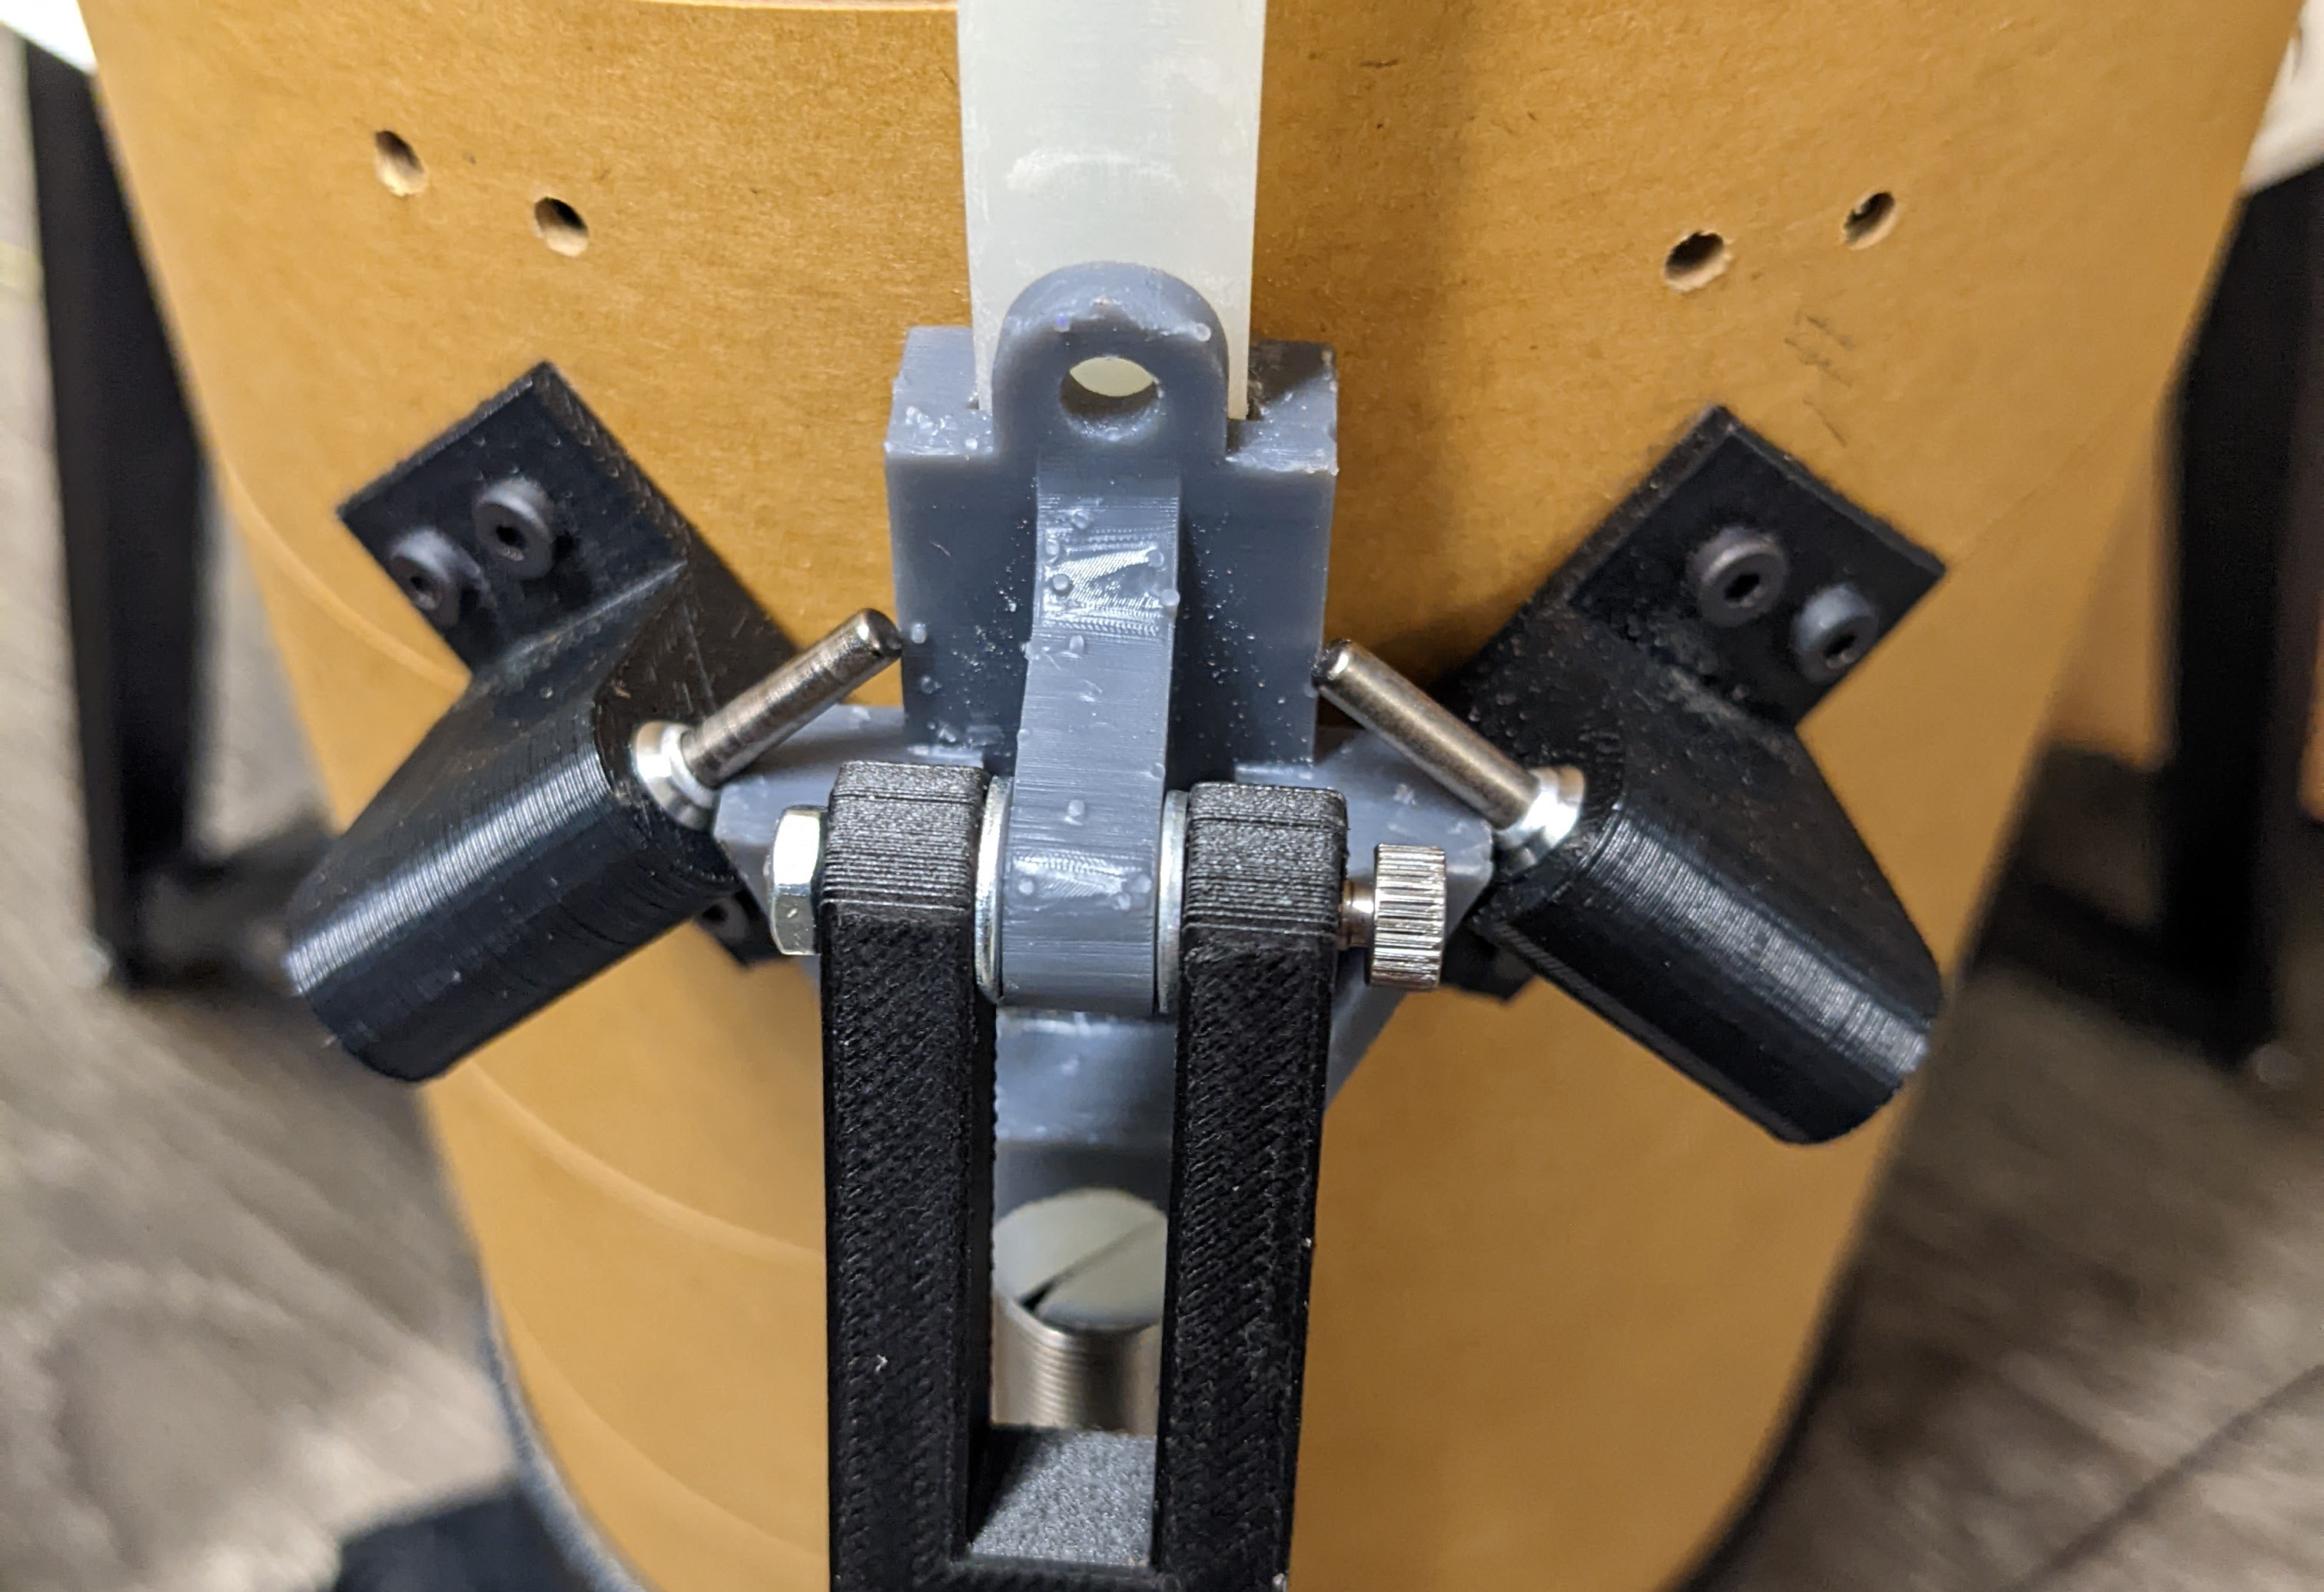
\includegraphics[width=0.75\textwidth]{src/figs/PinLocking.jpg}
    \caption{Pin Locking}
    \label{fig:lockpins}
\end{figure}


\subsection{Track and Carriage}

Rather than using purchased track and carriages, we designed and printed a custom track and carriage to better support our design. Commercial track's and carriages could directly mate to the outer radius of our rocket; hence, the carriage we designed has a slight curvature on its underside to provide a flush mount. Additionally, the track and carriage have a trapezoidal geometry to constrain motion in the normal and horizontal directions to allow for some play during deployment. 

The trapezoidal geometry of the carriage was designed to depress the press fit plungers as it slides past. It also includes a mount location for the primary strut and a hole for the pre-deployment pin to rest in. Both components were printed on the Formlabs resin printers in the RP Lab.

\section{Rocket Body}

The rocket tube diameter was decided based on the the inner most diameter that we could stow the arms, the core and the motors protruding from the arms. After optimization of that design, the team ended up with a value of almost exactly 6 inches.

\subsection{Material Selection}

Phenolic cardboard is a resin impregnated, spiral wrapped, and heat cured cardboard derivative with 5 times the compression strength of traditional cardboard. Fiberglass and carbon fiber have traditionally been used in amateur rocketry; however, these materials require an abundance of precaution during machining due to the inhalation hazard of microparticulates.

\subsection{Machining}

Making measurements and cuts on a cylindrical surface is inherently difficult. This difficulty was compounded by the fact that we require relatively tight positional tolerances and sheer number of holes we needed. In an effort to combat this we used converted the Solidworks model of our tube into a sheet metal part. We then created a 1:1 scale dimensioned drawing of this sheet metal component and printed it using a plotter in Mudd Library. This 2D drawing was wrapped around our rocket tube in preparation for machining. 

The first step of the machining process was to cut the slots out of the paper and make the markings on the rocket body. With the template still on the tube we drilled the holes through the paper. We then marked the bottom location of the template on the tube, removed the template, and cut to tube to length using a hacksaw. Finally, we used a dremel equipped with a cutoff wheel to hand-cut the arm slots. 

In hindsight, this method should have been paired with physical measurements to ensure the locations of the holes we drilled matched to have a higher degree of tolerance to match what we in the CAD measurements of the design. When assembling the lander, we had some serious hole misalignment which required lots of re-drilling. We suspect the error was due to the paper small crinkles when they did not when aligning it with the outside of the rocket tube. Even a 1mm misalignment makes a big difference with M3 screws.
